\documentclass[
12pt,
openany, %openright,			
oneside, %twoside,			%% twoside: para frente e verso ao imprimir
a4paper,			
english,			
brazil			        %% Idioma principal 
]{abntbibufjf}

%Arrumando as páginas e cabeçalhos
\usepackage[a4paper,width=150mm,top=25mm,bottom=25mm]{geometry}

\usepackage{fancyhdr}
\pagestyle{fancy}
\fancyhead{}
\fancyhead[CE]{\leftmark}
\fancyfoot{}
\fancyfoot[LE,RO]{\thepage}
\fancyfoot[LO,CE]{}
\fancyfoot[CO,RE]{Gabriel Eduardo de Lima Machado}


\usepackage[utf8]{inputenc}
\usepackage{graphicx}
\graphicspath{{images/}}
\usepackage[portuguese]{babel}
\usepackage{amsmath}
\usepackage{bigints}
\usepackage{tikz}
\usepackage{listings}
\usepackage{calc}
\usepackage{amsmath}
\usepackage{bigints}
\usepackage{xcolor}
\usepackage{float}
\usepackage{tocloft}
\usetikzlibrary{shapes,arrows}
\graphicspath{ {images/}{capitulos/chp3/images3/}{capitulos/chp2/images/} }

%citações
\usepackage[backend=bibtex,style=numeric]{biblatex}
\addbibresource{sample.bib}

\titulo{Implementação de técnicas adaptativas para análise de harmônicos e inter-harmônicos variantes no tempo} %%Por exemplo, Titulo da tese
% \subtitulo{: subt\'itulo do trabalho}  %% Retirar o primeiro ``%'' desta linha se for utilizar subtitulo. Deixar os dois pontos antes, em ``: subt\'itulo'' . 
\autor{Gabriel Eduardo de Lima Machado}
\autorR{Machado, Gabriel} %%Colocar o sobrenome do autor antes do primeiro nome do autor, separados por
\local{Juiz de Fora}
\data{2019} %%Alterar o ano se precisar
\orientador[Orientador:]{Marcelo Antônio Alves Lima} %%Se precisar, troque [Orientador:] por [Orientadora:]

\instituicao{Universidade Federal de Juiz de Fora}
\faculdade{Faculdade de Engenharia} %%Alterar, dentro de chaves {}, se precisar.
\programa{Engenharia Elétrica – Habilitação em Sistemas Eletrônicos} %%Alterar, dentro de chaves {}, se precisar.
\objeto{Trabalho de Conclusão de Curso}  %%Tese (Doutorado)
\natureza{Trabalho de Conclusão de Curso apresentado à Faculdade de Engenharia da Universidade Federal de Juiz de Fora, como requisito para obtenção do grau de Engenheiro Eletricista.} %%Trocar Matem\'atica por outro, se precisar.


%% Abaixo, prencher com os dados da parte final da ficha catalografica

\finalcatalog{1. Palavra-chave. 2. Palavra-chave. 3. Palavra-chave. I. Sobrenome, Nome do orientador, orient. II. Título.} %% Aqui fica 
% escrito a palavra ``T\'itulo'' mesmo, nao o do trabalho. Se tiver coorientador, os dados ficam depois dos dados 
%% do orientador (II. Sobrenome, Nome do coorientador, coorient.) e antes de ``II. T\'itulo'', o qual passa a ``III. T\'itulo''.

%% ---

\setlength{\parindent}{1.3cm}

\setlength{\parskip}{0.2cm}  

\setlength\afterchapskip{12pt}  


%% Iniciar o documento
\begin{document}
	
	%% ELEMENTOS PRE-TEXTUAIS
	
	%% Capa
	\inserecapa
	
	%% Folha de rosto
	\inserefolhaderosto
	
	
	%% Ficha catalografica. AO IMPRIMIR, DEIXAR NO VERSO DA FOLHA DE ROSTO.
	\inserecatalog  
	
	
	%% Folha de aprovacao
	\begin{folhadeaprovacao}
		
		\begin{center}
			{\chapterfont \bfseries \insereautor}
			
			\vfill
			\begin{center}
				{\chapterfont\bfseries\inseretitulo \inseresubtitulo}
			\end{center}
			\vfill
			
			\hspace{.45\textwidth}
			\begin{minipage}{.5\textwidth}
				\inserenatureza
			\end{minipage}%
			\vfill
		\end{center}
		
		Aprovado em: %%COLOCAR A DATA 
		
		\begin{center} BANCA EXAMINADORA \end{center}
		\assinatura{Prof. \insereorientador \ - Orientador \\ Universidade Federal de Juiz de Fora} 
		%  \assinatura{Professor Dr. \inserecoorientador \ - Coorientador \\ Universidade Federal de Juiz de Fora}
		\assinatura{Ex 1 \\  Universidade Federal de Juiz de Fora}
		\assinatura{Ex 2 \\ Universidade Federal de Juiz de Fora} 
		%  \assinatura{...} %%RETIRE O % E PREENCHA SE PRECISAR
		%  \assinatura{...}
		%  \assinatura{...}
		
		% \includepdf{ata.pdf} depois deverá ser substituído pela ata de defesa assinada
		
	\end{folhadeaprovacao}
	
	
	%% Dedicatoria. OPCIONAL. Retirar o ``%'' de cada das 4 linhas abaixo, caso queira.
	% \begin{dedicatoria} \vspace*{\fill} \centering \noindent
	%   \textit{ Dedico este trabalho ... (opcional)} 
	%   \vspace*{\fill}
	% \end{dedicatoria}
	
	
	%% Agradecimentos. OPCIONAL. CASO SEJA BOLSISTA, INSERIR OS DEVIDOS AGRADECIMENTOS.
	\begin{agradecimentos}
		
	Agradeço principalmente a meus pais e minha família, que são os maiores responsáveis por minha formação em qualquer que seja o âmbito e o principal suporte que tive durante todos os anos de estudo. 
	
	Agradeço também a meus grandes amigos de faculdade, pelos quais tenho um carinho muito especial, pois foram essenciais na jornada acadêmica além de torná-la muito mais divertida.
	
	Agradeço a todos professores, principalmente ao meu Orientador, que são as pessoas que fazem trabalhos como este serem possíveis.
		
		
		
		
	\end{agradecimentos}
	
	%% Epigrafe. OPCIONAL
	\begin{epigrafe}
		\vspace*{\fill}
		\begin{flushright}
			``Everything in this world is magic, except to the magician.''\\
			Hopkins, Anthony.
		\end{flushright}
	\end{epigrafe}
	
	
	%% RESUMOS
	
	%% Resumo em Portugu^es. OBRIGATORIO.
	\setlength{\absparsep}{18pt} 
	\begin{resumo}
		
		A estimação espectral não é um novo problema matemático ou de engenharia, há alguns séculos já se tenta escrever sinais como uma composição de diferentes frequências, entretanto este aparece de formas distintas nos mais diversos setores da tecnologia. Podemos citar sua importância em processamento de fala, área biomédica, na análise de eletroencefalogramas, identificação de sistemas, análise de vibrações e qualidade de energia. Este trabalho visa fundamentar teoricamente o problema em questão, implementar e avaliar técnicas já concebidas para sua solução, bem como apresentar variações e aplicações específicas. Serão utilizadas para tanto conhecidas técnicas de filtragem adaptativa com LMS e RLS, os chamados \textit{Phase-Locked-Loops} aliados a estruturas multitaxa e as ferramentas padrão da teoria de análise de sinais discretos no tempo. 
		
		
		
		
		Palavras-chave: Estimação Espectral, Filtros Adaptativos, Phase-Locked-Loop, Processamento Multitaxa, Banco de Filtros.
		%finalizadas por ponto e inicializadas por letra maiuscula.
		
	\end{resumo}



%% Resumo em Ingle^s
\begin{resumo}[ABSTRACT]
	\begin{otherlanguage*}{english}
		Spectral estimation is not a new mathematical or engineering problem, for centuries people have been trying to describe signals as a sum of sinusoidal frequencies.  However, this problem still shows up in different contexts on technology. We can highlight its relevance in signal processing, image processing, biomedical signals, system identification and modeling and power quality. This work aims to expose the fundamentals of the theory, to implement and evaluate well know techniques and present specific applications to this old problem. To reach this goal it is going to be used adaptive filtering methods as LMS and RLS, the so called Phase-Locked-Loops with multi rate structures and standard tools of discrete time signals analysis.  
		
		Key-words: Spectral Analysis, Adaptive Filtering, Phase-Locked-Loop, Multi Rate Processing, Filter Banks.
		
	\end{otherlanguage*}
\end{resumo}


%% Lista de ilustracoes. OPCIONAL.
\pdfbookmark[0]{\listfigurename}{lof}
\listoffigures*
\cleardoublepage


% Lista de tabelas. OPCIONAL. Retire o ``%'' de cada das 3 linhas seguintes, caso queira.
\pdfbookmark[0]{\listtablename}{lot}
\listoftables*
\cleardoublepage

% Lista de abreviaturas e siglas. OPCIONAL
\begin{siglas} %%ALTERAR OS EXEMPLOS ABAIXO, CONFORME A NECESSIDADE
	\item[AR]  Auto Regressivo
	\item[ARMA] Auto Regressivo Média Móvel 
	\item[DFT] Discrete Fourier Transform
	\item[DTFT] Discrete Time Fourier Transf
	\item[FIR] Finite Impulse Response
	\item[IIR] Infinite Impulse Response
	\item[NLMS] Normalized Least Mean Squere
	\item[PLL] Phase-Locked-Loop 
	\item[PLL-M] Phase-Locked-Loop Multitaxa
	\item[RLS] Recursive Least Mean Squares
	\item[STFT] Short Time Fourier Transform
	\item[TF] Transformada de Fourier
\end{siglas}

%% Lista de simbolos. OPCIONAL
\begin{simbolos} %%ALTERAR OS EXEMPLOS ABAIXO, CONFORME A NECESSIDADE
	\item[$ \forall $] Para todo
	\item[$ \in $] Pertence
	\item[$ \nabla $] Gradiente
	
\end{simbolos}

\chapter{Introdução}

\section{Análise Espectral}

Um dos conceitos mais antigos em análise de sinais é o de frequência. As funções senoidais, ou as exponencias complexas de modo geral, são fascinantes por possuírem diversas propriedades matemáticas interessantes, como por exemplo serem solução para diversas equações diferencias e quando são entrada de um sistema linear invariante no tempo, este sistema apresenta como saída um sinal da mesma classe da entrada, ou seja, outra exponencial complexa. O conceito de frequência sequer precisa estar ligado à series temporais. Em imagens ele também está presente na forma de frequência espacial. O próprio termo 'espectro' aparentemente foi introduzido por Newton enquanto estudava a decomposição da luz em diferentes cores. Tudo isso faz com que a decomposição de sinais em frequência seja um dos tópicos mais estudados em processamento de sinais. \cite{stoica2005spectral} \cite{castanie2013digital}.

É quase impossível dissociar o tópico da famosa transformada de Fourier, mas olhando da perspectiva do que é basicamente uma TF há diversas outras bases sobre as quais se pode projetar um sinal qualquer de modo a extrair determinadas características. Também é fato de que hoje esta análise se dá na maioria dos casos por meios digitais, dado o poder computacional que se tem à disposição atualmente e a fundamentação teórica sólida que dão teoremas como o famoso Teorema da amostragem de Nyquist-Shannon \cite{mitra2006digital} \cite{lago2002digital}. E ao final é o que utilizaremos basicamente neste trabalho, todo ele será baseado em análise digital de sinais e a maior parte com técnicas relacionadas à TF.

\section{Aplicações}

As aplicações da análise espectral são as mais diversas. Em processamento de imagens temos seu uso para encontrar fronteiras e comprimir arquivos, reduzindo seu tamanho e economizando banda de transmissão e espaço de armazenamento \cite{baxes1994digital}. 

Em processamento de fala, se pode utilizar para extrair características de fonemas, de modo a posteriormente classificá-los \cite{huang2001spoken}.

Em biomedicina, se pode usar para análise de eletrocardiogramas, e eletroencefalogramas na detecção de ondas alpha, beta, gamma e outras, que indicam determinadas atividades cerebrais e podem ser detectadas por análise espectral \cite{sornmo2005bioelectrical}.  

Além das demais citadas há uma área em especial que vem ganhando cada vez mais atenção e à qual se dedicam as simulações dos métodos que serão apresentados neste trabalho: a de qualidade de energia elétrica. Com o aumento constante de dispositivos não lineares ligados à rede elétrica, monitorar e filtrar harmônicos indesejados se torna indispensável. Atualmente tem-se diversas fontes de energia e características de cargas. A grande interligação que existe entre os sistemas de potência também trás preocupação de grades quedas no suprimento. Em resumo, o sistema de distribuição de energia elétrica está aumentando em complexidade, e desta maneira se fazem necessárias técnicas mais arrojadas para monitorá-lo e ajudar em seu controle \cite{dugan1996electrical}.

Observando atentamente o leitor se dará conta de que as simulações são em sua grande maioria feitas considerando uma componente fundamental em 60 Hz e principalmente os harmônicos ímpares até o 15º, que são os que normalmente aparecem em sistemas de potência. O trabalho se baseia nos seguintes artigos \cite{de2009pll} e \cite{chang2009two}, onde ambos os métodos propostos são concebidos com o intuito de analisar harmônicos e inter-harmônicos presentes comumente na rede elétrica.

\section{Divisão}

O capítulo 2 trata de uma fundamentação teórica e revisão bibliográfica (como indica o título) traçando os fundamentos da estimação espectral e conceitos de processamento de sinais. Neste capítulo discorre-se sobre a teoria por trás dos dois métodos mencionados anteriormente que são base deste trabalho, também estão presentes algumas demonstrações relevantes para o entendimento dos mesmos. 

O capítulo 3 fala especificamente do método PLL Multitaxa, suas características, os problemas que este visa solucionar e porque foi concebido desta maneira, mais alguns conceitos específicos que possam ter ficado de fora do capítulo 2. Estão incluídos resultados de simulações realizadas em MATLAB, na forma de figuras e tabelas.

O capítulo 4 trata da parte de estimação de frequências do método Adaline de dois estágios, e segue na mesma estrutura do capítulo 3: apresentamos sua construção, pontos fortes, fracos e resultados de simulação.

O capítulo 5 encerra o trabalho com um método unindo os dois anteriormente apresentados de forma complementar, utilizando o estágio de estimação de frequências presente no capítulo 4 para inicializar o método PLL Multitaxa. Ao final também são feitas algumas ponderações e proposições para trabalhos futuros.

\chapter{Revisão bibliográfica e Fundamentação Teórica}
%\documentclass[1indentpt,
%../main.tex]{subfiles}

\documentclass[a4paper, 12pt]{book}

\usepackage[portuguese]{babel}
\usepackage{graphicx}
\usepackage{amsmath}
\usepackage{bigints}
\usepackage{tikz}
\usetikzlibrary{shapes,arrows}

\begin{document}

Neste capítulo abordaremos as técnicas anteriormente mencionadas, que são o foco deste trabalho, PLL (Phase-Locked Loop), análise de prony, ADALINE e RLS (Recursive Least Mean Squares), bem como as convencionais DFT e STFT. Ressaltamos que esta será apenas uma abordagem superficial, não entraremos, portanto, com profundidade nos assuntos tratados.

\section{Análise espectral}
Análise espectral considera o problema de encontrar a energia de um sinal, finito, distribuída em função de frequência, o que pode ser feito com métodos paramétricos ou não paramétricos. Métodos paramétricos assumem conhecimento do modelo com o qual se gerou o sinal em análise. Por exemplo, em alguns capítulos, como o de análise de Prony, assumiremos que nosso sinal é composto unicamente por un número conhecido de exponenciais complexas amortecidas. Para solucionar um problema de estimação paramétrica, a única coisa que temos quer fazer (o que ainda não é fácil, na maioria dos casos) é encontrar os parâmetros supostos. Por outro lado, métodos não paramétricos se baseiam unicamente em transformações do domínio temporal para o domínio da frequência, utilizando filtros que nos dão a energia do sinal contida em uma determinada faixa do espectro, caso da DFT. Quando temos uma boa estimação de nosso modelo, os métodos paramétricos tendem a dar melhores resultados, enquanto que se pouco sabemos sobre o sinal analisado, ou se o mesmo não está bem modelado, os não paramétricos podem ser a melhor opção.

\indent Algumas vezes é conveniente tratar os sinais de maneira determinística, e o faremos neste trabalho, entretanto, como abordagem mais geral, se pode tratá-los com enfoque probabilístico, isto é: admitimos que não se pode de maneira alguma prever os valores assumidos por um sinal ao longo do tempo, mas se pode estimar suas características por meios estatísticos.
\indent Lembramos também que embora sinais reais sejam o caso mais comum na maioria das aplicações e em nosso caso são praticamente regra, não necessariamente o tratamento de sinais complexos é muito mais complicado. Apenas por uma questão de praticidade e para deixar o trabalho mais conciso, não demonstraremos os teoremas utilizados para entradas complexas quando não for necessário.[11]

\section{Densidade espectral de energia de um sinal determinístico}
Seja $y_c(t)$ um sinal contínuo no tempo e $y[n], \; n=0, \pm 1, \pm 2,...$  um sinal discreto tal que $y[n]=y_c(nT_s)$. Consideremos que $y[n]$ tem energia finita. Podemos dizer então que a DTFT de $y$ está definida como:

\begin{equation}
	Y(w)=\sum_{n=-\infty}^{+\infty}y[n]e^{-jwn}
\end{equation}

Onde $w$ é denominada frequência angular medido em radianos/segundo, e pode ser relacionada com seu valor físico da seguinte maneira $\bar{w}=wT_s$. A densidade espectral de potência do sinal $y(t)$ pode ser dada então por:
\begin{equation}
	S(w)=|Y(w)|^2
\end{equation}

Podemos interpretar este resultado de algumas formas, mas uma bem simples é lembrar que a DTFT de uma cossenoide é igual a soma de duas deltas refletidas no espectro de frequência:

\begin{equation}
	\sum_{n=-\infty}^{+\infty}cos(2\pi f \: n)e^{-jwn}= \pi \delta_{w}(2\pi f) + \pi \delta_{w}(-2\pi f) \;\; w \; \in [0,2 \pi]
\end{equation}

Uma relação muito parecida se estabelece no caso de uma senoide. Desta maneira, se imaginamos $yc(t)$ composta unicamente de uma soma de senoides, seu espectro fica muito bem explicitado com a equação XX.

Uma outra relação importante se dá utilizando a autocorrelação de $y[n]$:

\begin{equation}
r_y[k]=\sum_{n=-\infty}^{+\infty}y[n]y^*[n-k]
\end{equation}

\begin{equation*}
\sum_{k=-\infty}^{+\infty}r_y[k]e^{-jwk}=\sum_{n=-\infty}^{+\infty}\sum_{k=-\infty}^{+\infty}y[n]y^*[n-k]e^{-jwk}=
\end{equation*}
\begin{equation}
\begin{aligned}
\sum_{n=-\infty}^{+\infty}\sum_{k=-\infty}^{+\infty}y[n]y^*[n-k]e^{-jwn}e^{jw(n-k)}  = \\ \left[\sum_{n=-\infty}^{+\infty}y[n]e^{-jwn} \right]  \left[\sum_{s=-\infty}^{+\infty}y[s]e^{-jws} \right]^* = Y(w)Y(w)^*
\end{aligned}
\end{equation}

Vemos então que a DTFT da autocorrelação de um sinal é igual sua densidade espectral de energia.

\subsection{Densidade espectral de potência}

Para a maioria dos sinais com os quais lidamos, não temos um modelo puramente determinístico que os reproduza, não sabemos o valor exato que tomarão no futuro, e tampouco podemos estender seu valor até o infinito, ou analisar infinitas amostras do mesmo. Para os casos reais, é mais conveniente lidar com sequencias aleatórias ao longo do tempo, em que cada realização da sequência tem associada uma distribuição de probabilidade (até o momento de sua ocorrência, quando esta colapsa em algum valor). Para a maioria dos casos, consideraremos que estamos lidando com processos estacionários em sentido amplo[12]. Para este trato aleatório, não é regra que nossos sinais tenham energia finita, mas é possível ao invés disso, estimar sua densidade de potência.

\indent Assumamos agora que $y[n]$ é uma sequência de variáveis aleatórias, com o mesmo domínio da sequência anterior, e que $E[y[n]]=0$ para todo $n$. Tendo todas as variáveis aleatórias média nula. A função de correlação de $y[n]$ está definida como:

\begin{equation}
 r_y[k]=E[ y[n] \: y[n-k]^*]
\end{equation}
  
\indent Definimos então a densidade espectral de potência como:

\begin{equation}
\phi (w)=\sum_{k=-\infty}^{+\infty}r_y[k]e^{-jwk}
\end{equation}

\indent Uma segunda definição para a PSD (\textit{Power Spectrum Density}) pode ser dada como a DTFT do sinal com o número amostras tendendo ao infinito da seguinte forma:

\begin{equation}
\phi(w)=\lim_{N\rightarrow \infty}\frac{1}{N}\left|\sum_{k=0}^{N-1}y[k]e^{-jwk}  \right|^2
\end{equation}

\indent Ambas definições são equivalentes. Veremos mais adiante que uma das formas principais de se calcular a PSD é por meio de estimações da função de autocorrelação do sinal em questão.


\subsection{Periodograma e correlograma}

Uma forma bastante simples de estimar a PSD seria:

\begin{equation}
\hat{\phi_p}(w)=\frac{1}{N}  \left|\sum_{k=0}^{N-1}y[k]e^{-jwk}  \right|^2
\end{equation}

A qual chamamos periodograma. Outra forma poderia ser:

\begin{equation}
\hat{\phi_c}(w)=\sum_{k=-(N-1)}^{N-1}r_y[k]e^{-jwk}
\end{equation}

A qual chamamos correlograma. Dois estimadores para a autocorrelação serão apresentados abaixo, considerando $n=0,1,2,..., N-1$:

\begin{equation}
\hat{r}_y(k)=\frac{1}{N-k}\sum_{n=k}^{N-1}y[n] \: y^*[n-k]
\end{equation}

\begin{equation}
\hat{r}_y(k)=\frac{1}{N}\sum_{n=k}^{N-1}y[n] \: y^*[n-k]
\end{equation}

O primeiro estimador é chamado estimador padrão não viesado, e o segundo é um estimador viesado. Lembramos que é assim chamado (viesado) um estimador cuja esperança não é o que visa estimar. Fato é também que $\hat{\phi_p}$ é igual a $\hat{\phi_p}$ se $\hat{r_y}$ for estimada com estimador viesado.

\indent Muitas vezes o estimador em XX é preterido ao de XX, porque para muitos sinais a autocorrelação para valores grandes de k (valores considerados longe do 0) é muito baixa, e portanto não ajudaria fazer a correção do fator de normalização. Entretanto esse pode não ser bem o nosso caso, porque estaremos considerando nossos sinais muitas vezes como senoides puras, as quais apresentam correlação em trechos periódicos. Em realidade, não iremos sequer adentrar muito em estimadores de correlação. Partiremos logo para análise de métodos relacionados a DFT. As vantagens e desvantagens destes métodos todos podem ser vistos à luz de processos estocásticos, ou pela análise das características do método em si. Tentaremos mostrar um pouco de ambos, os utilizando da maneira que for mais conveniente. 
%===================DFT==========================
\section{DFT}
A transformada discreta de Fourier (DFT) de uma sequência discreta {x[n]} de tamanho N é definida como[5]:
\begin{equation}
X[k]=\sum_{n=0}^{n=N-1} x[n]e^{(-2jnk\pi/N)}\;,\;k=0,1,2,...,N-1
\end{equation}

Podemos dizer que a sequência X[k] é a DFT de x[n]. As duas sequências tem o mesmo tamanho, e X[k] representa o mapeamento das frequências de x[n] supondo estas estacionárias e com período igual ao analisado. Sendo Ts o tempo de amostragem da sequência x[n], temos a seguinte relação:
\begin{equation}
R_s=\frac{1}{T_sN}
\end{equation}
\indent Onde Rs é igual a resolução de X[k]. Temos o mapeamento dado como:
\begin{equation}
f_k=R_s k\;,\;k=0, 1, 2,...,N/2
\end{equation}
\indent Percebemos que a DFT age como uma série de Fourier, onde valores absolutos de X[k] são vistos como a amplitude de uma determinada frequência múltipla da componente fundamental f1, que é igual a resolução Rs. Para um sinal contendo apenas harmônicos de f1, e eventualmente algum valor médio, podemos extrair perfeitamente seus valores de amplitude e fase. Entretanto, para um sinal que possui componentes inter-harmônicos, não é possível fazer o mesmo. Neste caso ocorre o chamado \textit{espalhamento}. Já se pode notar algumas deficiências da DFT. Também temos problemas caso não seja amostrado um período exato do sinal analisado, ou um múltiplo inteiro de um período, podendo a DFT levar a crer, por exemplo, que existe um valor médio no sinal, e outros conteúdos equivocados. Este fenômeno é denominado \textit{spectral leackage}[5]. 

\indent Como a DFT pressupõe um sinal estacionário, ela não é adequada para análise de sinais variantes no tempo. Para tanto podemos utilizar de uma DFT de janela deslizante. Para uma janela de tamanho N, temos:

\begin{equation}
X[k,m]=\sum_{n=0}^{N-1} x[m-n]e^{(-2jnk\pi/N)}\;,\;k=0,1,2,...,N-1
\end{equation}

\indent Desta forma, para cada m>N, temos uma janela de tamanho N onde será analisado o sinal. Existem algoritmos mais eficazes para efetuar este tipo de cálculo de forma recursiva, sem precisar calcular toda a DFT como se estivéssemos diante de uma amostra completamente nova:
\begin{equation}
X[k,m]=C\{X[k,m-1]e^{j2\pi k/N}+(x[m]-x[m-N])e^{j2\pi k/N}\}\;,\;k=1,2,...,N/2
\end{equation}

\indent C=1/N para k=N/2 e igual a 2/N para os demais valores. O valor de k foi restringido levando-se em conta a simetria dos sinais reais.[Não sei de onde veio essa equação, vou ver depois]

\indent Pode-se usar diferentes tipos de janelas além da anterior, que é uma janela quadrada, onde todos os termos da sequência tem igual peso no cálculo da DFT. O uso de outras janelas ajuda na amenização do \textit{leackage}. Algumas janelas estão expostas abaixo.

Janela triangular:
\begin{equation}
w_{tri}(n)=1-\frac{|2n-N+1|}{N-1}\;,\;0\leq n \leq N-1
\end{equation}

Janela de Hamming:
\begin{equation}
w_{hm}(n)=0.54-0.46cos(\frac{2\pi n}{N-1})\;,\;0\leq n \leq N-1
\end{equation}

\indent O uso deste tipo de janelamento atenua eventuais descontinuidades nas extremidades do sinal, auxiliando na medição dos parâmetros. Aplicar uma janela ao sinal significa deslizar a sequência formada por $w$ por x[n], multiplicando termo a termo. Desta forma poderíamos reescrever a equação XXX como:
\begin{equation}
X[k,m]=\sum_{n=0}^{n=N-1} x[m-n]*w(n)*e^{(-2jnk\pi/N)}\;,\;k=0,1,2,...,N-1
\end{equation}

\indent podemos ver nas figuras o efeito da aplicação do janelamento.

\begin{figure}[h]
	\centering
	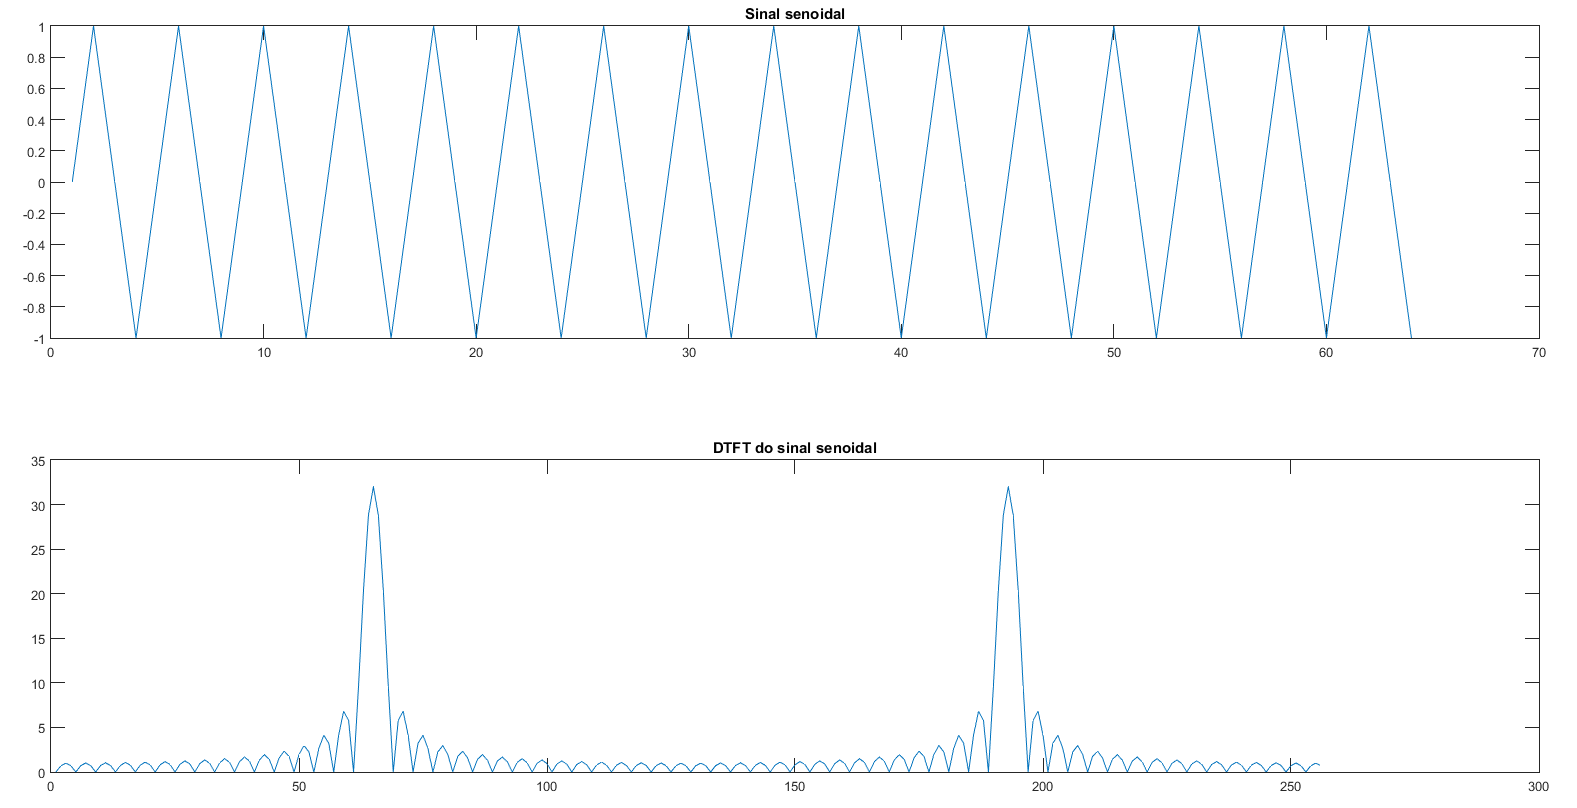
\includegraphics[width=0.9\textwidth]{../figuras/f5.png}
	\caption{legenda aqui}
	\label{fig:f5}
\end{figure}

\begin{figure}[h]
	\centering
	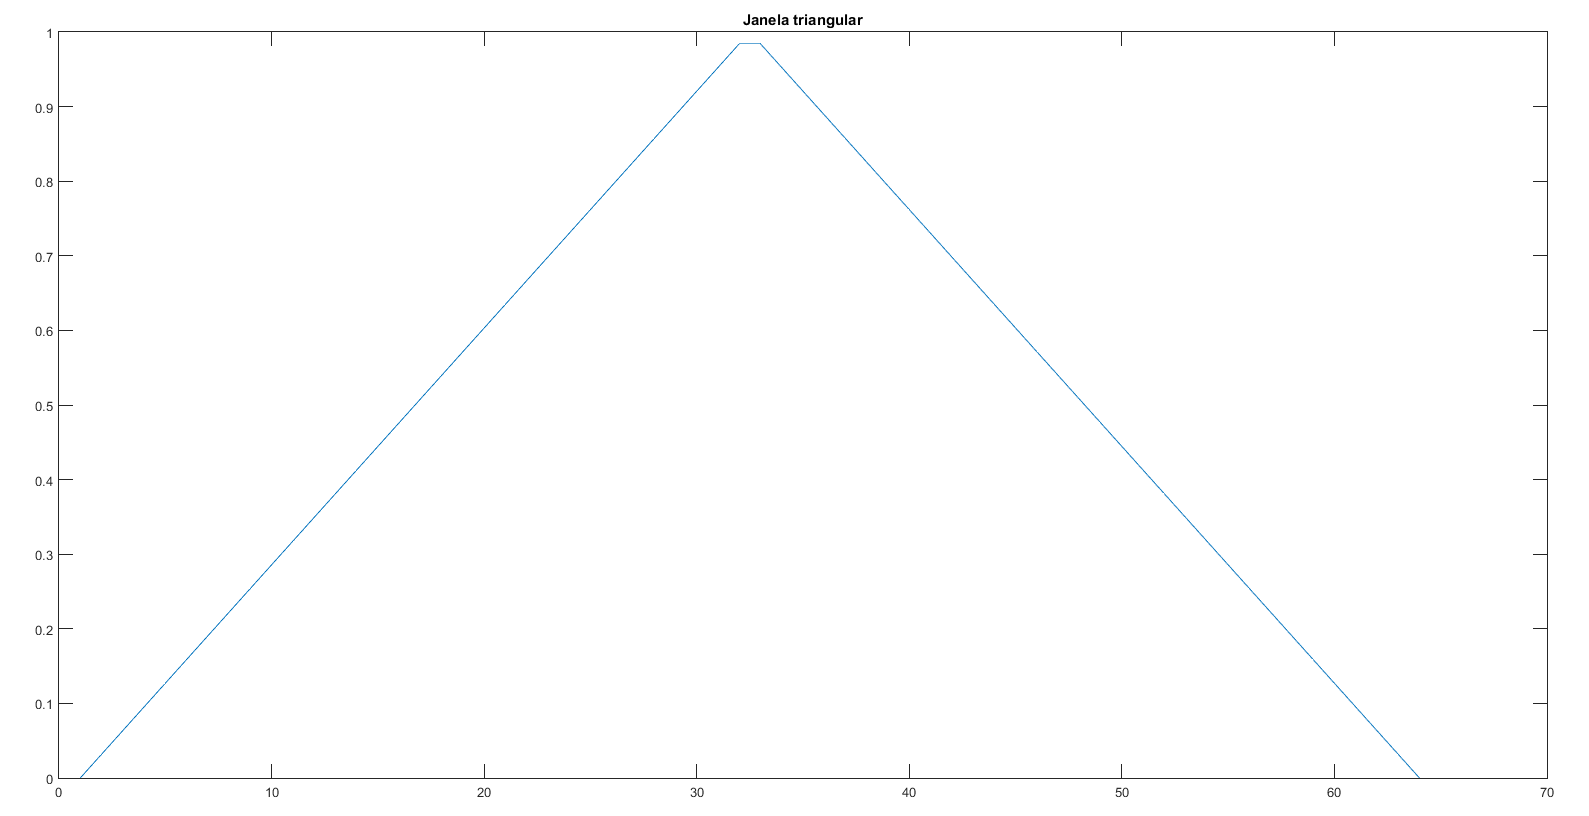
\includegraphics[width=0.9\textwidth]{../figuras/f4.png}
	\caption{legenda aqui}
	\label{fig:f4}
\end{figure}

\begin{figure}[h]
	\centering
	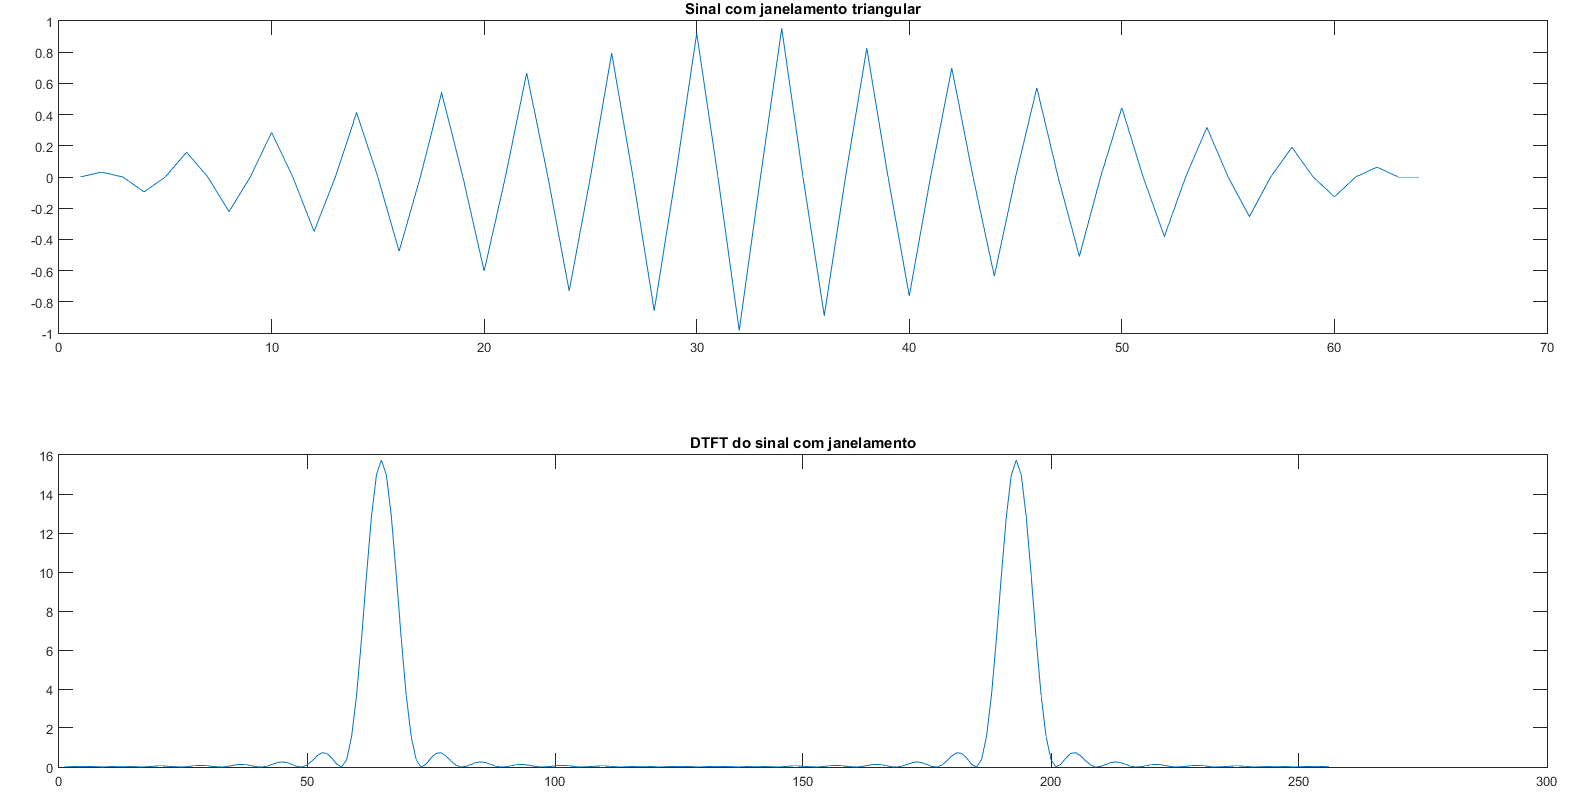
\includegraphics[width=0.9\textwidth]{../figuras/f3.png}
	\caption{legenda aqui}
	\label{fig:f3}
\end{figure}

\begin{figure}[h]
	\centering
	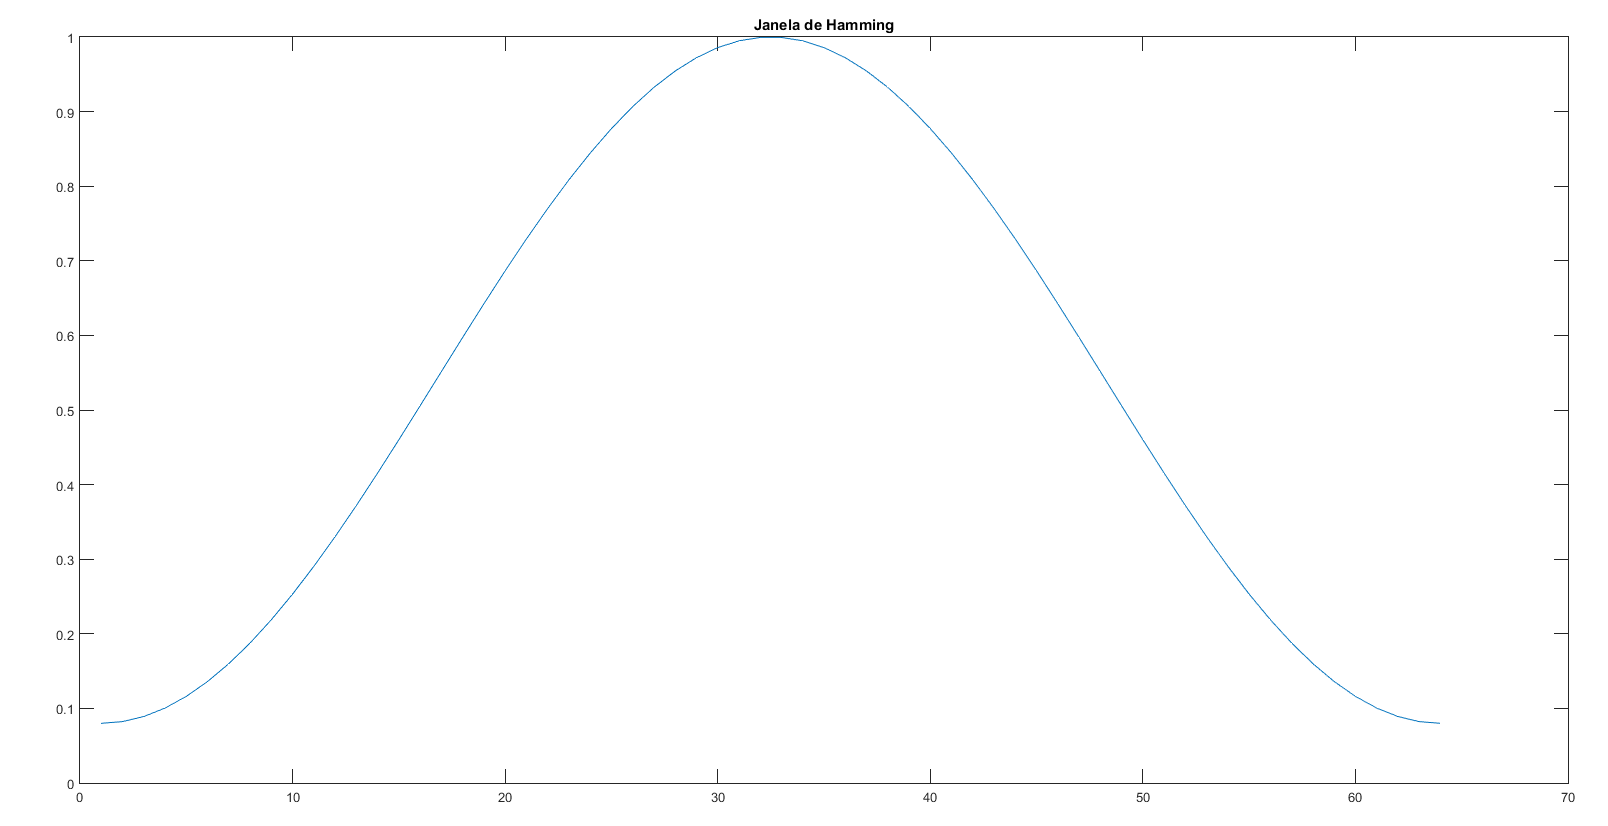
\includegraphics[width=0.9\textwidth]{../figuras/f2.png}
	\caption{legenda aqui}
	\label{fig:f2}
\end{figure}

\begin{figure}[h]
	\centering
	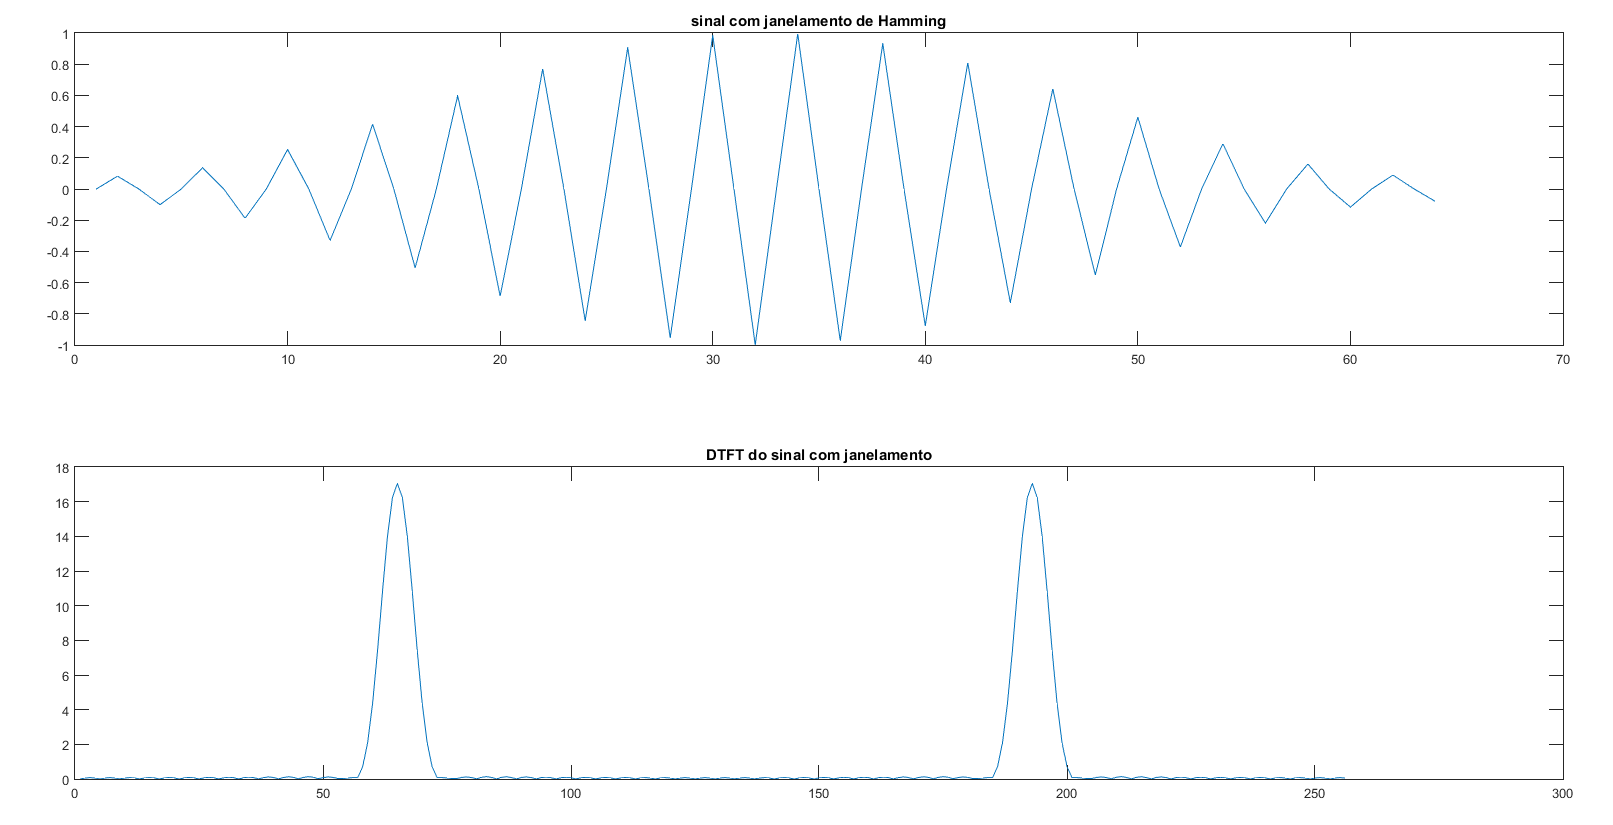
\includegraphics[width=0.9\textwidth]{../figuras/f1.png}
	\caption{legenda aqui}
	\label{fig:f1}
\end{figure}

\section{Análise de Prony}
A análise de Prony foi desenvolvida em 1795 de modo a explicar a espanção de gases. Ela se assemelha em parte a DFT, entretanto se propõe a ajustar uma soma de exponenciais complexas amortecidas a uma sequência de dados igualmente espaçados, ao passo de que a DFT apenas estima as exponeciais complexas e em subdivisões predeterminadas da frequência de amostragem. A análise de prony não é somente uma técnica de análise de sinais, mas também de indentificação de sistemas amplamente utilizada em sistemas de potência, área biomédica, processamento de fala, decaimento radioativo entre outas. 
A análise de Prony é conhecida por não se comportar muito bem quando um sinal contém ruído, a técnica não faz distinção entre sinal e ruído, e também ajusta as exponenciais ao ruído presente.
Seguindo o proposto em [3], temos o seguinte para um sinal $y[k]$ imaginando M exponenciais para se ajustarem a 2M amostras, respeitando o teorema da amostragem:

\Large
\begin{equation}
y[k]=\sum_{m=1}^{M}A_me^{(\alpha_m+j2\pi f_m)(k-1)\Delta t +j\sigma_m}\;,\;k=1,2,...,2M
\end{equation}
\normalsize

\indent Onde $fm$ é a frequência das exponenciais, $\Delta t$ é o tempo de amostragem, $\alpha _m$ é o coeficiente de amortecimento, e $\sigma _m$ é o ângulo de defasagem. Para o método proposto, estamos apenas interessados em saber quais são as frequências presentes no sinal. Se imaginamos nosso sistema sendo auto regressivo (AR) de ordem M, temos que em qualquer instante de $k$ é possível prever o valor $y[k]$ considerando apenas as M amostras anteriores deste mesmo sinal. Podemos então montar uma equação de diferenças, que neste caso também é um modelo de predição linear[4]:

\begin{equation}
y[k]=\sum_{m=1}^{M}a_m y[k-m]
\end{equation}

É sabido que exponenciais complexas são soluções para tal modelo. Se tivermos em mãos os valores dos coeficientes $a$ podemos montar o polinômio característico da equação e as raízes deste polinômio (exponenciais complexas) são soluções para nosso problema. De posse dos coeficientes $a$ devemos então encontrar as raízes do polinômio seguinte:
\begin{equation}
P(z)=z^M-a_1z^{M-1}-...-a_Mz^0
\end{equation}

\indent Como os coeficientes $a$  são reais, as raízes complexas estão em pares complexos conjugados, desta maneira cada par complexo representa uma possível senóide já que $cos(wt)=\frac{e^{jwt}+e^{-jwt}}{2}$:
\begin{equation}
f_m=atan(Im\{z_m\}/Re\{z_m\})2\pi fs
\end{equation}

\indent Onde $_zm$ é uma das raízes e $fs$ é a frequência de amostragem.
\indent Reparemos que as frequências $f_m$ são frequências de possíveis soluções do sistema, não necessariamente elas estarão presentes. Qualquer combinação linear dessas senióides também é solução do sistema AR planteado. Para encontrar a forma da solução real, é  necessário fazer uso das condições iniciais conhecidas de nosso sistema. No caso, as próprias amostras $y[k]$ as quais temos acesso.

\indent Os coeficientes de amortecimento $\alpha_m$ são o módulo das raízes complexas que encontramos. E se alguma raíz não é complexa, isto somente significa que uma exponencial é solução para nossa equação.
\begin{equation}
\alpha_m=|zm|
\end{equation}
\subsection{Solução do modelo de predição linear}

Existem diversas formas de solucionar um modelo deste tipo, apresentaremos algumas opções abaixo[9]:

\subsubsection{Sistema linear}

Conhecendo os valores $y[k]$ que são amostras de nosso sistema analisado, podemos montar um sistema linear considerando a equação anterior:
\begin{equation}
y[k]=\sum_{m=1}^{M}a_m y[k-m]
\begin{bmatrix}
y[k-1] & y[k-2] & \dots & y[k-M] \\
y[k-2] & y[k-3] & \dots & y[k-M-1] \\
\vdots & & & \vdots\\
y[k-M] & y[k-M-1] & \dots & y[k-2M+1]
\end{bmatrix}
\begin{bmatrix}
a_1 \\ a_2 \\ \vdots \\ a_M
\end{bmatrix}
=
\begin{bmatrix}
y[k] \\ y[k-1] \\ \vdots \\ y[k-M+1]
\end{bmatrix}
\end{equation}

Ou de forma simplificada:

\begin{equation}
\boldsymbol{Y_k}\boldsymbol{a}=\boldsymbol{y_k}
\end{equation}

A forma mais simples de resolver este sistema é inverter a matriz $\boldsymbol{Y_k}$:

\begin{equation}
\boldsymbol{a}=\boldsymbol{Y_k}^{-1}\boldsymbol{y_k}
\end{equation}

Um dos problemas com esta solução é que ela é computacionalmente custosa, já  que não está implementada de maneira recursiva, mas pior que isso é o fato de que normalmente temos ruído em nosso sistema, e desta maneira estamos ajustando os valores de $\boldsymbol{a}$ ao ruído também, o que em geral não é o desejado, e em nosso caso, certamente não é. Desta forma, cada vez que calculamos o vetor $\boldsymbol{a}$, ele pode sair completamente diferente do anterior, nos levando a estimações equivocadas. Modelando $y[k]$ como:
\begin{equation}
y[k]=\sum_{m=1}^{M}a_m y[k-m]+\xi_k
\end{equation}

Em que $\xi_k$ é ruído branco, temos um modelo estocástico de nosso sinal, que nos possibilita pensar em soluções mais arrojadas. 

\subsection{Filtros adaptativos}

\indent O Elemento linear adaptativo, ou filtro FIR adaptativo, também chamado de ADALINE, é uma rede neural artificial composta de uma única camada e com função de ativação linear. Sendo $\boldsymbol{x}$ as entradas, $\boldsymbol{w}$ os pesos, $b$ o valor de bias, o ADALINE pode ser implementado matricialmente da seguinte maneira:


\begin{equation}
y=
\begin{bmatrix}
x_{1} & x_{2} & x_{3} & \dots & x_{n} \\
\end{bmatrix}
\begin{bmatrix}
w_{1}  \\
w_{2}  \\
\vdots  \\
w_{n} 
\end{bmatrix}
+ b = \boldsymbol{x}^T \, \boldsymbol{w}+b
\end{equation}

\begin{figure}[h]
	\centering
	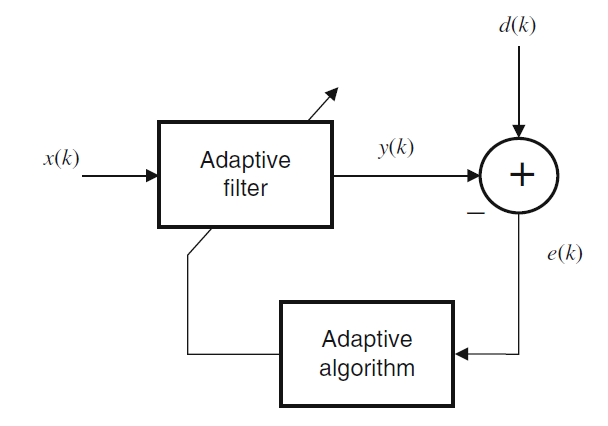
\includegraphics[width=0.9\textwidth]{../figuras/fA.png}
	\caption{legenda aqui}
	\label{fig:filtroAdaptativo}
\end{figure}

\indent Filtros adaptativos são considerados sistemas não lineares, portanto a análise de seu comportamento é mais complexa que de a filtros com coeficientes fixos. Por outro lado, pelo fato de serem auto-projetados, por um ponto de vista mais prático, eles podem ser considerados menos complicados que os convencionais em termos de projeto[6].

\indent O desenho usual de um filtro adaptativo pode ser visto na figura \ref{fig:filtroAdaptativo}, onde $k$ é o número da iteração, $x(k)$ é a entrada do filtro, $y(k)$ é o sinal de saída, $d(k)$ é o valor de referência e $e(k)=d(k)-y(k)$ é o valor de erro, necessário para o algoritmo de adaptação do filtro. O algoritmo de adaptação é o prcesso usado para ajustar os coeficientes do filtro de modo a minimizar o erro de acordo com os critétios preestabelecidos. A escolha do algoritmo determina muitos aspectos do processo de adaptação, como a existência de soluções subótimas e complexidade computacional.

\subsection{Adaptação via gradiente descendente}

Uma das formas mais antigas e consagradas de otimizar uma função dentro dos métodos clássicos é seguir a direção do gradiente desta função, com relação as variáveis de interesse, para atualizar os valores destas variáveis de forma iterativa.

Consideremos um sistema discriminado pela série temporal $u[n] \space n=0,1,2..$ e um filtro de resposta impulsiva real $w_0, w_1 ... w_{M-1}$:
\begin{equation}
y[n]=\sum_{k=0}^{M-1}u[n-k]w_k
\end{equation}
Todo este desenvolvimento pode ser feito de maneira bastante similar considerando entradas complexas e filtros com coeficientes complexos, mas por questões de simplicidade estaremos focando no caso em que ambos são reais. Imaginemos que desejamos que a saída deste filtro seja uma outra série temporal igualmente real $d[n]$, assim nosso erro seria:
\begin{equation}
e[n]=d[n]-y[n]    
\end{equation}

Considerando o caso de $u$ estocástico, $e[n]$ é uma variável aleatória. Gostaríamos então de minimizar a esperança de $e^2[n]$, definimos então nossa função de custo:
\begin{equation}
J=E[e^2[n]]=E[(d[n]-y[n])^2]   
\end{equation}

Definindo nosso operador gradiente $\nabla_k$:
\begin{equation}
\nabla_k J=-2 E[e[n]u[n-k]]   
\end{equation}

Se queremos encontrar o ótimo com relação a esta função de custo, $\nabla_k J$ deve ser igual a zero para todo $k$, como a esperança do produto de duas variáveis aleatórias é sua correlação, $u[n-k]$ e $e[n]$ devem estar descorrelacionadas para todo $k$. A este resultados chamamos princípio da ortogonalidade. Um corolário deste princípio é que $y$ também deve ser ortogonal, ou descorrelacionada com $e[n]$.

\indent É mais conveniente para nó trabalhar com a notação matricial destes resultados. Ao vetor coluna que contém as variáveis aleatórias $u[n-k]$, de k=0 a K=M-1, lhe chamamos $\boldsymbol{u}_n$, ao vetor de coeficientes $w$, igualmente:

\begin{equation*}
\boldsymbol{u}_n=
\begin{bmatrix}
u[n] & u[n-1] & \dots & u[n-M+1]
\end{bmatrix}^T
\end{equation*}
\begin{equation*}
\boldsymbol{W}_n=
\begin{bmatrix}
w_0 & w_1 & \dots & w_{M-1}
\end{bmatrix}^T
\end{equation*}
Desenvolvendo nossa equação anterior, podemos obter:

\begin{equation}
\nabla J=-2 E[e[n]\boldsymbol{u}_n]=2E[\boldsymbol{u}_n\boldsymbol{U}^{T}_n\boldsymbol{W}-d[n]\boldsymbol{u}_n]   
\end{equation}

Desta última equação, destacamos que $E[d[n]\boldsymbol{U}_n]$ é o vetor de correlação cruzada entre $d[n]$, que chamaremos de $\boldsymbol{r_{du}}$ e as amostras atrasadas do sinal de entrada.Destacamos também que $E[\boldsymbol{U}_n\boldsymbol{U}^{T}_n]$, a qual chamaremos $\boldsymbol{R_{uu}}$, é a matriz MxM de autocorrelação do mesmo sinal. Sendo assim, escrevemos agora:

\begin{equation}
\boldsymbol{R}_{uu}\boldsymbol{w}-\boldsymbol{r}_{du}=0
\end{equation}

De onde podemos concluir que o vetor coeficientes ótimos $\boldsymbol{w}_{opt}$ é:

\begin{equation}
\boldsymbol{w}_{opt}=\boldsymbol{R}_{uu}^{-1}\boldsymbol{r}_{du}
\end{equation}

Se $u$ é um processo estacionário em sentido amplo, então podemos coletar amostras suficientes para fazer uma boa estimação das matrizes acima, encontrando assim um filtro muito mais apropriado para nossos propósitos. Desta maneira, é possível estimar o conteúdo espectral de $u$ com precisão. Reparemos que este método não é propriamente um gradiente escendente já que encontramos a solução em um passo apenas.

\indent A solução acima tem sua utilidade, entretanto, se a natureza do sinal mudar, não teremos mais uma boa aproximação do mesmo, neste caso, é melhor resolver estas equações de forma recursiva, de modo que o filtro possa se adaptar constantemente à mudanças ocorridas.  

\subsection{O algoritmo LMS}

Para atualizar o vetor de pesos $\boldsymbol{w}_n$ na direção oposta a do gradiente, definimos um coeficiente de aprendizagem $\mu$. A cada iteração vamos fazer o seguinte:

\begin{equation*}
\boldsymbol{w}_{n}=\boldsymbol{w}_{n-1} - \mu \nabla J
\end{equation*}
\begin{equation}
\boldsymbol{w}_{n}=\boldsymbol{w}_{n-1} + \mu(\boldsymbol{r}_{du}-\boldsymbol{R}_{uu} \boldsymbol{w}_{n+1})
\end{equation}

O que diferencia o LMS de outros métodos de gradiente descendente é a forma de estimar as matrizes $\boldsymbol{R}_{uu}$ e $\boldsymbol{r}_{du}$. Vamos estimâ-las da seguinte forma:

\begin{equation}
\boldsymbol{\hat{R}}_{uu}=\boldsymbol{u}_n \boldsymbol{u}_{n}^T
\end{equation}
\begin{equation}
\boldsymbol{\hat{r}}_{du}=\boldsymbol{u}_n d[n]
\end{equation}

O que pode soar uma heresia, mas faz sentido se pensarmos que apenas temos M amostras de sinal.

\subsection{O algoritmo NLMS}

Uma melhoria no algoritmo anterior pode ser proposta. Se multiplicamos a parte que está entre parênteses na equação XX:

\begin{equation}
\boldsymbol{w}_{n}=\boldsymbol{w}_{n-1} + \mu \boldsymbol{R}_{uu}^{-1}(\boldsymbol{r}_{du}-\boldsymbol{R}_{uu} \boldsymbol{w}_{n+1}) = \boldsymbol{w}_{n-1} + \mu(\boldsymbol{w}_{opt} - I \boldsymbol{w}_{n-1}) = \boldsymbol{w}_{opt}
\end{equation}

Em teoria, nosso algoritmo convergiria em apenas uma iteração. Resta apenas o empecilho de que estimar tal matriz. Com estimador que tínhamos antes isto não é possível, porque a matriz estimada $\boldsymbol{\hat{R}}_{uu}$ não é inversível por ser o produto de dois vetores. Mas podemos fazer uma aproximação da forma $\boldsymbol{\hat{R}}_{uu} + \boldsymbol{I} \epsilon$. Que certamente é inversível e pode nos dar uma inversa útil, para valores pequenos de $\epsilon$. E após alguma álgebra[10], que pode ser encontrada em [9], chegamos ao seguinte:

\begin{equation}
\boldsymbol{w}_{n}=\boldsymbol{w}_{n-1} + \mu \frac{\boldsymbol{u}_{n}}{|\boldsymbol{u}_{n}|^2 + \epsilon }(d[n]-\boldsymbol{u}_{n} \boldsymbol{w}_{n-1}) =\boldsymbol{w}_{n-1} + \mu \frac{\boldsymbol{u}_{n}}{|\boldsymbol{u}_{n}|^2 + \epsilon }e[n]
\end{equation}

A este algoritmo chamamos LMS normalizado, ou NLMS. Há ainda o estudo de convergência para valores pequenos de $\mu$, que também pode ser encontrado em [6][9], tanto para o LMS quanto para o NLMS. Mas de modo geral o NLMS deve convergir respeirada todas as condições estabelecidas anteriormente e escolhendo valores de $\mu<1$.

\subsection{RLS}

\indent O método RLS (\textit{Recursive Least Squares}), ou mínimos quadrados recursivo, é um método de adaptação que visa a minimização da soma dos quadrados da diferença entre o sinal de referência e o sinal de saída do filtro em questão (o erro), assim como os anteriormente mencionados. O RLS pode ser obtido a partir do LMS (\textit{Least Mean Squares}), e é conhecido por possuir rápida convergência, tendo boa performance em sistemas variantes no tempo, como o caso de nosso interesse. Isto vem ao custo de certa complexidade computacional aliada a problemas de estabilidade[6].

\indent Voltando ao modelo do filtro adaptativo da seção anterior, havíamos feito uma estimação bastante simplória de $\boldsymbol{R}_{uu}$ para o LMS, e um pouco mais desenvolvida no NLMS, agora imaginemos uma outra: nos casos anteriores somente aproveitávamos as M últimas amostras de nosso sinal para cada iteração, mas se por exemplo fazemos uma média das $\boldsymbol{R}_{uu}^{(k)}$ nos aproximamos mais da matriz verdadeira de autocorrelação. Podemos escolher então um novo estimador para $\boldsymbol{R}_{uu}$:

\begin{equation}
\boldsymbol{S}_{d}^{-1}=\boldsymbol{\hat{R}}_{uu}=\frac{1}{k+1}\sum_{i=0}^{k}\lambda^{k-i}\boldsymbol{U}_i\boldsymbol{U}_i^*
\end{equation}

\indent Esta definição em realidade é uma média ponderada em uma série geométrica, e se $\lambda<1$ as últimas amostras contam mais que as primeiras. Reparemos que se $\lambda=1$ temos um estimador consistente da matriz. A $\lambda$ chamamos fator de esquecimento.


\indent Outra forma de se chegar ao RLS é por sua função objetivo dada por:

\begin{equation}
\xi(k)=\sum_{i=0}^{k}\lambda^{k-i}\varepsilon^2(i)
=\sum_{i=0}^{k}\lambda^{k-i}[d(i)-\boldsymbol{x}(k) \boldsymbol{w}(k)]
\end{equation}

\indent Onde $\varepsilon$ é o erro a posteriori no instante $i$. Lembrando da equação XX deduzida anteriormente, podemos estimar a matriz $\boldsymbol{R}_{uu}$ de forma recursiva, para evitar cálculos desnecessários, e melhor que isso, sua inversa também pode ser calculada de maneira recursiva, o que é mais importante para nós. A inversa pode ser substituída na expressão obtida para o NLMS. A dedução no entanto não nos interessa tanto no trabalho, ela pode ser encontrada em [6] e [9]. Ficamos com o resultado final:

\Large
\begin{equation}
\boldsymbol{\phi}^{-1}_k=\lambda^{-1}\Bigg[\boldsymbol{\phi}_{k-1}-\frac{\boldsymbol{\phi}_{k-1}\boldsymbol{u}^T_k\boldsymbol{u}_k\boldsymbol{\phi}_{k-1}}{\lambda+\boldsymbol{u}_k\boldsymbol{\phi}_{k-1}\boldsymbol{u}^T_k}\Bigg]
\end{equation}
\normalsize

\indent Os pesos então podem ser atualizados da seguinte maneira:

\begin{equation}
\boldsymbol{w}_{n}=\boldsymbol{w}_{n-1} +  \boldsymbol{\phi}_{n}^{-1}e[n] \boldsymbol{u}_{n}
\end{equation}

\indent Uma recomendação de inicialização de $\boldsymbol{\phi}_0$ é $\boldsymbol{\phi}_0=\delta \boldsymbol{I}$, sendo $\delta$ o inverso da potência estimada do sinal.



%% ============== PLL ========================



\section{PLL}

\indent Um Phase Locked Loop digital, assim como sua versão analógica, visa determinar os parâmetros de um processo estocáscico como uma onda senoidal. Desta forma o PLL tenta extrair parâmetros de Amplitude, fase e frequência. Temos diversas variantes digitais e analógicas[7], a variante utilizada neste trabalho foi proposta por Ziarani em 2004[8]. Uma breve demostração será realizada abaixo.
\indent Seja $u(t)$ uma função variante no tempo, e $y(t)=Asin\phi(t)$ um sinal periódico senoidal sendo A a amplitude do sinal e $\phi(t)$ sua fase, tendo este sinal uma frequência constante, podemos escrever $\phi(t)=wt+\delta$, sendo $w$ igual a frequência e $\delta$ um valor de fase constante. Podemos escrever de maneira mais geral:

\begin{equation}
u(t)=\sum_{i=0}^{\infty}A_i sin\phi_i(t)\space+\space n(t)
\end{equation}

Onde $n(t)$ representa um distúrbio, como um ruído. Na realidade, todos os parâmetros podem variar com o tempo, é conveniente escrever então um conjunto $\Psi(t)=[A(t), w(t), \delta(t)]$ o qual contém todos os parâmetros de um possível sinal $y(t)$.

Definimos a função $d$:
\begin{equation}
d^2(t,\Psi(t))=[u(t)-y(t,\Psi(t))]^2=e^2(t)
\end{equation}

Assim sendo o conjunto $\Psi(t)$ ótimo o que minimiza a função $d^2$ que adotaremos como função de custo $J(\Psi(t),t)$. Os parâmetros $\Psi(t)$ podem ser estimados por meio de gradiente descendente.

\begin{equation}
\frac{d\Psi(t)}{dt}=-\boldsymbol{\mu}\frac{\partial J(\Psi(t),t)}{\partial \Psi(t)}
\
\end{equation}

\begin{equation}
\boldsymbol{\mu}=
\begin{bmatrix}
m_1 && 0 && 0 \\
0 && m_2 && 0 \\
0 && 0 && m_3
\end{bmatrix}
\end{equation}

Com $\frac{d\Psi(t)}{dt}$ denotando o vetor na dierção do qual são atualizados os valores de $\Psi(t)$ a cada iteração. E $\boldsymbol{\mu}$ a matriz diagonal contendo as constantes de atualização referentes a cada parâmetro. Como estaremos lidando com estimações agora, usaremos a notação $\hat{\Psi}(t)$:

\begin{equation}
\begin{bmatrix}
\frac{d\hat{A}(t)}{dt} \\
\frac{d\hat{w}(t)}{dt}\\
\frac{d\hat{\delta}(t)}{dt}
\end{bmatrix}
=-\boldsymbol{\mu}
\begin{bmatrix}
\frac{\partial e^2(t)}{\partial \hat{A}} \\
\frac{\partial e^2(t)}{\partial \hat{w}} \\
\frac{\partial e^2(t)}{\partial \hat{\delta}}
\end{bmatrix}
\end{equation}

Podemos obter então o seguinte:
\begin{equation}
\frac{d\hat{A}(t)}{dt}=2m_1e(t)sin(\int_{0}^{t}\hat{w}(\tau)d\tau\space+\space\hat{\delta}(t))
\end{equation}
\begin{equation}
\frac{d\hat{w}(t)}{dt}=2m_2e(t)\hat{A}(t)tcos(\int_{0}^{t}\hat{w}(\tau)d\tau\space+\space\hat{\delta}(t))
\end{equation}
\begin{equation}
\frac{d\hat{\delta}(t)}{dt}=2m_3e(t)\hat{A}(t)cos(\int_{0}^{t}\hat{w}(\tau)d\tau\space+\space\hat{\delta}(t))
\end{equation}
\begin{equation}
\frac{d\hat{\phi}(t)}{dt}=\hat{w}(t)+\frac{\hat{\delta}(t)}{dt}
\end{equation}

Por conta do fator temporal $t$ que aparece solto na equação referente a $\hat{w}$, esse sistema é variante no tempo, o que o torna instável. No entanto uma solução heurística é substituir $t$ por uma constante $m4$, que pode ser absorvida pela constante $m2$, tornando o sistema invariante no tempo e fazendo com que este sistema de equações seja útil na prática. Desta maneira obtemos o seguinte:
\begin{equation}
\frac{d\hat{A}(t)}{dt}=2\mu_1e(t)sin(\int_{0}^{t}\hat{w}(\tau)d\tau\space+\space\hat{\delta}(t))
\end{equation}
\begin{equation}
\frac{d\hat{w}(t)}{dt}=2\mu_2e(t)\hat{A}(t)tcos(\int_{0}^{t}\hat{w}(\tau)d\tau\space+\space\hat{\delta}(t))
\end{equation}
\begin{equation}
\frac{d\hat{\phi}(t)}{dt}=\hat{w}(t)+2\mu_3e(t)\hat{A}(t)cos(\int_{0}^{t}\hat{w}(\tau)d\tau\space+\space\hat{\delta}(t))
\end{equation}

Usando o método \textit{Euler Forward}:

\begin{equation}
A[n+1]=A[n]+\mu_1T_s e[n]sen(\phi(t))
\end{equation}
\begin{equation}
w[n+1]=w[n]+\mu_2T_s e[n]cos(\phi(t))
\end{equation}
\begin{equation}
\phi[n+1]=\phi[n] + T_s w[n] + \mu_3T_s e[n]cos(\phi(t))
\end{equation}

Desta forma obtemos o conjunto de equações discretas que utilizaremos para rastrear frequências no restante do trabalho.

\begin{figure}[h]
	\centering    
	\def\svgwidth{\columnwidth}
	\input{pll_basico.pdf_tex}
	\caption{Convergência do PLL com a presença de apenas a fundamental}
	\label{fig:your image label}
\end{figure}

%=============Multitaxa================

\section{Processamento Multitaxa}

Em determinadas situações, é desejável alterar a taxa de amostragem de um sinal para realizar certos tipos de processamento. Por exemplo, veremos em alguns resultados nas próximas sessões que o algoritmo PLL descrito anteriormente é sensível a taxa de amostragem em relação a frequência rastreada, portanto é conveniente mantê-la mais ou menos constante. Também veremos que processar sinais na taxa necessária para abranger todo o espectro que se quer analisar é extremamente custoso computacionalmente e não é garantia de melhores resultados. Por isso deve-se considerar o uso de uma estrutura multitaxa que diminua a frequência base.

\indent Analisaremos a seguir as implicações de um abaixamento na frequência de amostragem:

\subsection{Downsampling}

Uma estrutura downsampling tem a forma seguinte:

\tikzstyle{int}=[draw, fill=blue!20, minimum size=2em]
\tikzstyle{init} = [pin edge={to-,thin,black}]

\begin{center}
\begin{tikzpicture}[node distance=2.5cm,auto,>=latex']
\node [int] (a) {$M_k \downarrow$};
\node (b) [left of=a,node distance=2cm, coordinate] {a};
%\node [int, pin={[init]above:$p_0$}] (c) [right of=a] {$\frac{1}{s}$};
\node [coordinate] (end) [right of=b, node distance=4cm]{};
\path[->] (b) edge node {$x(k)$} (a);
\draw[->] (a) edge node {$y(k)$} (end) ;
\end{tikzpicture}
\end{center}


Representamos a estrutura como um sistema que reproduz em sua saída apenas amostras onde $k$ é múltiplo de $M_k$. Podemos escrever $y[n]=x[nM_k] \; n=1,2,3...$ Considerando que $x[k]$ foi amostrado com a frequência de Nyquist $fs$, o efeito final é o mesmo que se tivéssemos amostrado $x$ com $fs/M_k$, podemos dizer que vamos observar aliasing em nosso resultado final. Haverá portanto sobreposição no espectro de frequência referente a $X(w)$ quando analisarmos $Y(w)$. Entretanto, é possível prever onde estarão localizadas as componentes espectrais presentes no sinal completo que estamos subamostrando, e embora não possamos saber exatamente qual é o valor correspondente as frequências originais, podemos saber no mínimo qual é sua soma.

\indent Uma demonstração formal dos efeitos observados pode ser encontrada em[5], aqui faremos uma abordagem mais intuitiva. Imaginemos uma componente espectral de $x[k]$ referente a $w_0$. Imagine que fazemos uma subamostragem neste sinal, e agora sua frequência de amostragem que era $f_s$ se torna $f_s/M_k$. Agora, se $w_0<f_s/(2Mk)$ essa as componentes dessa frequência não saem do lugar, elas continuam onde estavam anteriormente. Isso não significa que seu espectro não seja alterado nas frequências mais baixas que a nova taxa de amostragem, somente quer dizer que elas sofrem interferência no mesmo lugar onde estavam antes. Agora, se a frequência de interesse é maior que a nova frequência de amostragem dividida por 2, então ela não poderá de forma alguma ser encontrada no mesmo local, pois simplesmente não há como visualizá-la com DFT ou DTFT. Mas então onde vão parar essas frequências? Bom, onde pararia qualquer uma que sofre aliasing. Ela dá voltas no círculo de frequências. O circulo de frequências sempre vai de 0 a $2\pi$, e as frequências sempre caminham nele no sentido anti-horário. Para cada vez que a frequência de interesse (a qual chamaremos $f_i$) for maior que $fs$, a frequência em questão dá uma volta no círculo. Um algoritmo simples será apresentado quando expusermos o método do PLL multitaxa, mas por hora podemos saber que o ângulo referente à nova frequência será o resto da divisão $f_i/f_s$ e multiplicamos por $2\pi$. 

\begin{figure}[h]
	\centering
	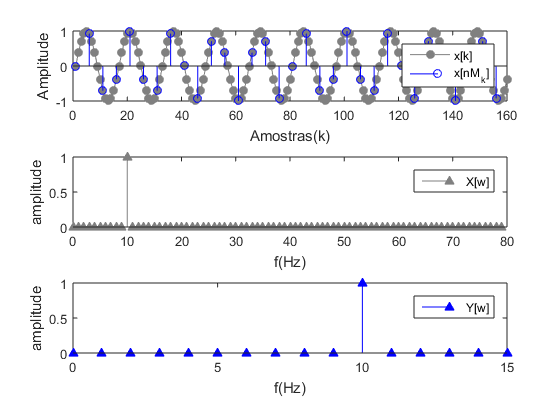
\includegraphics[width=0.9\textwidth]{../figuras/downsample.png}
	\caption{Downsampling para $f_s=160Hz$, $f_0=10Hz$, $M_k=5$}
	\label{fig:f5}
\end{figure}

\begin{figure}[h]
	\centering
	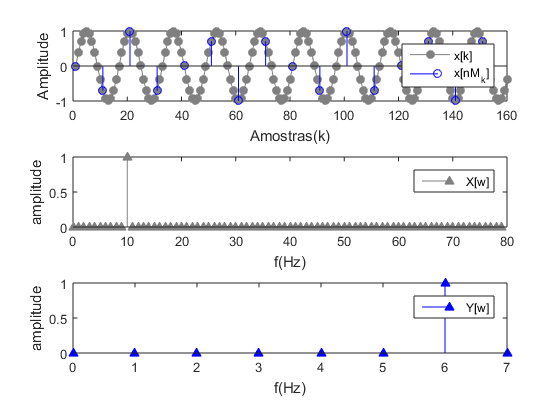
\includegraphics[width=0.9\textwidth]{../figuras/downsample2.png}
	\caption{Downsampling para $f_s=160Hz$, $f_0=10Hz$, $M_k=10$}
	\label{fig:f5}
\end{figure}

No exemplo da figura XX, temos $fs=160Hz$ e $M_k=5$, nossa frequência de interesse é 10Hz, a frequência de amostragem depois da subamostragem seria ainda maior que $2f_i$, então ela não se move, como observado na figura. Entretanto, no caso de $M_k=10$ a coisa muda, calculando:

\begin{equation}
w_i=rest(f_i \: M_k, \: f_s)2\pi
\end{equation}



\end{document}

\chapter{Estrutura PLL-Multitaxa}
% para incluir imagens:
% inkscape -D -z --file=simple_pll_harmonicos.svg --export-pdf=simple_pll_harmonicos.pdf --export-latex
	
Como visto na seção referente ao PLL, esse método é capaz de minimizar o erro quadrático médio entre um sinal $y(t)$ e uma componente senoidal para ao menos um mínimo local. Neste capítulo ganhará forma uma estrutura reunindo o PLL e o processamento multitaxa com o objetivo de reduzir a complexidade computacional e conseguir um algoritmo mais versátil. 

\section{Desenpenho do PLL}
Nas figuras seguintes pode-se observar como converge o algoritmo em diferentes situações, todas foram simuladas para um sinal de 180 V de amplitude e constantes 300, 500, e 6, com frequência de amostragem igual a 7680 Hz, partindo de condições inicias $f_i=60 Hz$ e $A=0$. Percebe-se pela simulação que o algoritmo converge rapidamente mesmo com ruído, entretanto, na presença de harmônicos com a mesma quantidade de energia, a convergência já é bastante comprometida. Ainda assim, em valor médio, a estimação se mostra correta. Conclui-se que é possível estimar harmônicos diretamente com o algoritmo PLL obtido, entretanto é conveniente aliá-lo a outras técnicas para que se diminua o erro da estimação. Os resultados das simulações podem ser vistos nas figuras \ref{fig:PLL_conv1} e \ref{fig:PLL_conv2}.

\begin{figure}[h]
	\centering    
	\def\svgwidth{\columnwidth}
	\input{images/simple_pll_harmonicos.pdf_tex}
	\caption{Convergência na presença do 3º e 5º harmônicos; SNR=10 dB}
	\label{fig:PLL_conv1}
\end{figure}

\begin{figure}[h]
	\centering    
	\def\svgwidth{\columnwidth}
	\input{images/pll_ruido.pdf_tex}
	\caption{Convergência na presença de ruído; SNR=10 dB}
	\label{fig:PLL_conv2}
\end{figure}

\section{Banco de filtros}

\indent A solução encontrada em \cite{de2009pll} para parte dos problemas anteriormente citados é o uso de um pré-processamento com filtros passa-banda, para melhorar a relação sinal ruído, e posteriormente subamostragem, para diminuir a complexidade computacional, de modo também que não seja necessário mudar as constantes do algoritmo.

\indent O conjunto de filtros utilizado é uma cascata de dois filtros IIR com a seguinte função de transferência:

\begin{equation}
H_{bp}(z)=\frac{1-\alpha}{2}\frac{1-z^{-2}}{1-\beta (1-\alpha) z^{-1} + \alpha z^{-2}}
\label{eq:filtro}
\end{equation}
\begin{equation}
\beta=cos(w_0)
\label{eq:w0 filtro}
\end{equation}

\indent O parâmetro $\alpha$ modifica a seletividade do filtro e está entre 0 e 1, para que este seja estável. Quanto mais próximo de 1, mais seletivo é o filtro. O parâmetro $\beta$ modifica a frequência central do filtro de acordo com a equação \ref{eq:w0 filtro}, onde $w_0$ é a frequência normalizada de acordo com a amostragem.

\indent Este filtro é uma boa escolha por alguns motivos:
\begin{itemize}
	\item Ele rechaça completamente a componente DC do sinal.
	\item Tem atraso de fase nulo na frequência central.
	\item É paramétrico, suas características dependem dos parâmetros $\alpha$ e $\beta$, os quais modificam propriedades muito específicas do filtro, sendo então muito fácil utilizá-lo e modificá-lo em tempo real.
\end{itemize}

\begin{figure}[h]
	\centering    
	\def\svgwidth{\columnwidth}
	\input{images/banco_de_filtros.pdf_tex}
	\caption{Características do filtro com $w_0$=0.25}
	\label{fig:your image label}
\end{figure}

\indent Tem-se talvez como única desvantagem o atraso de grupo que é máximo para a frequência central, e quanto mais seletivo é o filtro, maior é esse atraso. Deve-se também ter atenção com a frequência de amostragem, pois quanto maior, menos seletivo um mesmo $\alpha$ seria. Se por exemplo, se mantém $\alpha$ e aumenta $f_s$, frequências que antes estavam normalizadas mais longe de nossa frequência central anterior, agora estariam mais próximas, por assim dizer. Dessa forma quanto maior é $f_s$ mais seletivo deve ser o filtro para a separação das mesmas frequências. Isso acaba se tornando um jogo de balanceamento destes parâmetros, pois como vimos anteriormente, um $\alpha$ maior também eleva o atraso de grupo, entretanto se tem mais amostras em menos tempo devido ao aumento em $f_s$. Todos estes efeitos estão muito bem descritos por J. Rodrigues em seu trabalho \cite{carvalho2008estimaccao}. Ao final utilizaremos $\alpha = 0.975$ e dois filtros em cascata para o restante das simulações.

\section{Uso da estrutura multitaxa}

Depois de passado pelo filtro passa-banda, pode-se realizar a subamostragem do sinal, uma vez que em tese eliminamos os harmônicos mais distantes quase que completamente, e estes não interferirão na estimação. Dentro revisão bibliográfica foi discutido o perfil desta interferência e também como encontrar a posição de uma frequência depois de esta sofrer aliasing. Agora é feita a exposição do algoritmo em C de uma função simples capaz de calcular esta frequência, que pode ser até mais explicativo que o texto anterior:

\lstinputlisting[language=c]{capitulos/chp3/algoritmo.c}

A função recebe como argumentos a frequência de amostragem Fs, a frequência rastreada \text{f\_init}, e o ponteiro para a variável flag, que indica se a frequência encontrada estava no semicírculo positivo, quando vale 1, ou negativo, quando vale -1 ($\theta<\pi$ ou $\theta>\pi$). É importante guardar esta informação porque necessitamos dela para recuperar a frequência original estimada. 

\begin{figure}[h]
	\centering    
	\def\svgwidth{\columnwidth}
	\input{images/circulo_freq.pdf_tex}
	\caption{Círculo de frequências}
	\label{fig:freq_circ}
\end{figure}

\indent É possível observar na figura \ref{fig:freq_circ} a localização de duas frequências f1 e f2 no círculo. Suponhamos que a frequência de amostragem é $f_s=240 \:Hz$, $f_2=\frac{240}{2} \frac{3}{4} \: Hz = 90 \: Hz$ e $f_2=\frac{240}{2} \frac{4}{3} \: Hz = 160 \: Hz$, encontramos facilmente suas colocações no círculo utilizando o algoritmo citado. Agora reparemos que diferentes frequências serão mapeadas nas mesmas posições do círculo, por exemplo $f_1=\frac{240}{2} \frac{11}{4} \: Hz = 330 \: Hz$ também é mapeada no mesmo ângulo, então não existe uma função inversa que devolva as frequências mapeadas para seus valores reais. 

\indent Também é importante se atentar ao fato de que quando se aumenta $f_1$ levemente, se está aumentando sua frequência aparente, mas quando se faz o mesmo com $f_2$ se está diminuindo sua frequência aparente. Por isso é importante guardar a variável 'flag'. Ela diz se acréscimos positivos em frequência aparente condizem à acréscimos ou decréscimos na frequência real, e uma vez que não existe uma função inversa que nos devolva a frequência real dada a aparente, deve-se utilizar da variação na estimação aparente e o valor inicial mapeado para recuperar a estimação real.

\indent Uma coisa que se deve ter em mente é que algumas frequências se localizarão muito próximas a zero, e terão frequência aparente muito pequena. Isso dificulta muito a análise, é desejável testar a localização antes de iniciar o algoritmo e fazer uma mudança no valor de subamostragem caso necessário.

\begin{equation}
\hat{f}=f_{init}+\Delta f_{aparente}\, flag
\end{equation}

\section{Variação da frequência central do banco de filtros}

\begin{figure}[h]
	\centering    
%	\def\svgwidth{\columnwidth}
	\def\svgscale{0.7}
	\input{images/esquema_pll.pdf_tex}
	\caption{Esquema multitaxa PLL}
	\label{fig:esquema_pll}
\end{figure}

\indent A estrutura multitaxa consiste em passar o sinal de entrada $x(t)$ pelo banco de filtros, sub-amostrar e passar este sinal para os respectivos PLLs. Como o filtro utilizado é bastante seletivo, a frequência estimada deve controlar o banco de filtros centrando a frequência corretamente. A maneira mais básica de realizar este controle seria alimentar o banco diretamente com as frequências obtida no PLL, entretanto este método é inviável. Vimos na seção sobre o algoritmo PLL utilizado que este é altamente não linear, e complexo de se analisar a convergência. Fazer uma realimentação deste tipo muda o sistema e pode torná-lo instável, ou prejudicar sua convergência. A alternativa encontrada por J. Rodrigues \cite{carvalho2008estimaccao}  é utilizar a média das últimas $L$ estimações, assim o filtro passa-banda se move de maneira mais suave e não prejudica tanto o PLL. Desta maneira:
   
\begin{equation}
w_0[k]=\frac{1}{L} \sum_{i=k-L+1}^{k}\hat{w}[i]
\end{equation}

\indent Uma outra opção é fazer a estimação com uma série geométrica, ou soma convexa, que pode ser calculada de forma recursiva:
 
\begin{equation}
w_{0}[k]=w_{0}[k-1](1-\lambda) + \lambda \hat{w}[k]
\label{eq:w0 filtro}
\end{equation}

Onde $\lambda$ é uma constante entre 0 e 1. \\

\begin{figure}[h]
	\centering    
	%	\def\svgwidth{\columnwidth}
	\def\svgscale{1}
	\input{images/media_direto.pdf_tex}
	\caption{Comparação entre o método de média (com 24 amostras) e o de alimentação direta}
	\label{fig:esquema_pll}
\end{figure}

\begin{figure}[h]
	\centering    
	%	\def\svgwidth{\columnwidth}
	\def\svgscale{1}
	\input{images/geometrico_media.pdf_tex}
	\caption{Comparação entre o método de média (com 24 amostras) e o geométrico ($\lambda=0.9$)}
	\label{fig:esquema_pll}
\end{figure}

\indent Simulando as três opções, a alimentação direta da estimação realmente se mostra mais instável, e com maior tempo de convergência, enquanto que o método geométrico em geral é levemente mais estável e de mais rápida convergência que o de média, além de ser mais fácil de computar. Todos foram testados para as mesmas constantes do exemplo anterior, amplitude de 180 V e 60 Hz iniciais, a constante de subamostragem escolhida foi $M_k=16$. Depois de 1 segundo de simulação, é aplicado um degrau na frequência de -2 Hz. Também é passado um filtro média móvel de 16 amostras nos resultados finais de $\hat{w}$ e $\hat{A}$.

\section{Síntese da estrutura PLL Multitaxa}

\begin{enumerate}
	\item Passamos o sinal por um banco de filtros;
	\item Abaixamos a frequência em $M_k$ amostras;
	\item Calculamos a frequência aparente $f_a$ da componente a rastrear;
	\item Inicializamos o PLL com esta $f_a$ e a guardamos para recompor a original;
	\item Fazemos as estimações de $w$ e $A$, usamos a equação \ref{eq:w0 filtro} e utilizamos a série geométrica para realimentar o banco de filtros com a frequência calculada.
\end{enumerate}

\section{Simulações}

Para as simulações computacionais foram seguidos determinados critérios:

\begin{itemize}
	\item Convergência em amplitude: Foram consideradas as últimas 32 estimações, assim que a média do erro quadrático destas fosse menor que 4e-4 (que é um erro menor que 2\% do sinal), consideramos que o algoritmo convergiu.
	\item O mesmo para a convergência em amplitude, mas com umbral de 1e-4.
	\item Os cálculos de erro quadrático médio são feitos considerando o valor das estimações depois de 1 segundo. Quando o algoritmo já convergiu.
\end{itemize}

Os parâmetros da simulação são $f0=60Hz$, 128 pontos por ciclo de $f0$, $Fs=7380 \,Hz$, $\alpha=0.975$ e dois filtros em cascata no banco. A constante de subamostragem é 16, para todos os harmônicos e inter-harmônicos. A amplitude da fundamental é 180 V, e para todos os harmônicos suas amplitudes são a da fundamental dividido pela ordem do respectivo harmônico. Foi passado um filtro média móvel de ordem 16 em todas as estimações de modo a suavizar a visualização dos resultados.

\subsection{Harmônicos ímpares}

\indent Abaixo estão os resultados para a simulação com os harmônicos ímpares de 1 a 15. Verificamos algumas coisas:
\begin{itemize}
	\item o valor de offset para a fundamental é relativamente grande, e isto se explica principalmente pela subamostragem, uma vez que alguns harmônicos não são completamente atenuados se sobrepõe à fundamental. Isso poderia ser melhorado com o aumento da seletividade do filtro, entretanto já discutimos os problemas que isto pode ocasionar. Seu uso ou não depende da natureza do problema em questão.
	\item o erro em frequência é em geral mais baixo que o de amplitude. E também é seu tempo de convergência.
	\item o tempo de convergência é difícil de prever, não é certo que os harmônicos de ordem mais elevada ou os de maior energia convergirão mais rapidamente que os demais.
	\item o algoritmo se comporta muito bem com ruído, principalmente a estimação de frequência.
\end{itemize} 
\begin{table}[H]
	\begin{tabular}{|p{2.5cm}|p{2.5cm}|p{2.5cm}|p{2.5cm}|p{2.5cm}|}
		\hline
		Harmônico & Erro em frequência (\%) & Erro em amplitude (\%) &
		Tempo de convergência W (s) & tempo de convergência Amp. (s)\\
		\hline
		1  & 6,14E-07 & 1,344 & 0,144 & 0,098 \\
		3  & 2,08E-06 & 1,427 & 0,150 & 0,135 \\
		5  & 2,16E-06 & 1,338 & 0,035 & 0,088 \\
		7  & 3,05E-05 & 1,441 & 0,090 & 0,194 \\
		9  & 1,60E-05 & 0,913 & 0,035 & 0,090 \\
		11 & 4,93E-05 & 1,146 & 0,035 & 0,221 \\
		13 & 2,01E-04 & 0,136 & 0,035 & 0,090 \\
		15 & 4,57E-03 & 0,126 & 0,035 & 0,327 \\
		\hline
	\end{tabular}
\caption{Tabela para a simulação sem ruído}
\end{table}


\begin{table}[H]
	\centering
	\begin{tabular}{|p{2.5cm}|p{2.5cm}|p{2.5cm}|}
		\hline
		Harmônico & MSE em frequência (\%) & MSE em amplitude (\%)\\
		\hline
		1  & 4,21E-05 & 2,32E-04 \\
		3  & 6,05E-07 & 3,16E-04 \\
		5  & 4,23E-07 & 5,42E-04 \\
		7  & 3,70E-07 & 1,01E-03 \\
		9  & 5,56E-07 & 1,45E-03 \\
		11 & 3,26E-07 & 1,96E-03 \\
		13 & 7,37E-07 & 3,65E-03 \\
		15 & 7,76E-07 & 4,56E-03 \\
		\hline
	\end{tabular}
	\caption{Tabela para a simulação com ruído ($\sigma ^2$=10)}
\end{table}

\begin{figure}[H]
	\centering    
	%	\def\svgwidth{\columnwidth}
	\def\svgscale{1}
	\input{images/harm15_ruido.pdf_tex}
	\caption{Convergência do 15º harmônico na presença de ruído}
	\label{fig:esquema_pll}
\end{figure}

\begin{figure}[H]
	\centering    
	%	\def\svgwidth{\columnwidth}
	\def\svgscale{1}
	\input{images/harm15_deg.pdf_tex}
	\caption{Convergência do 15º harmônico com degrau em frequência}
	\label{fig:esquema_pll}
\end{figure}

\subsection{Inter-harmônicos}

Foram simuladas estimações com inter-harmônicos, seguindo as mesmas prescrições do caso anterior. Vemos que os tempos de convergência não são muito afetados, entretanto o erro quadrático médio para a fundamental aumenta um pouco. Isto se deve a um leve batimento que o harmônico 3.2 causa na fundamental, fazendo com que a estimação oscile um pouco. Contudo, se olhamos uma média grande o suficiente destas estimações, podemos nos livrar do batimento.

\begin{figure}[H]
	\centering    
	%	\def\svgwidth{\columnwidth}
	\def\svgscale{1}
	\input{images/batimento.pdf_tex}
	\caption{Batimento observado na fundamental}
	\label{fig:esquema_pll}
\end{figure}

\begin{figure}[H]
	\centering    
	%	\def\svgwidth{\columnwidth}
	\def\svgscale{1}
	\input{images/harm64.pdf_tex}
	\caption{Convergência do inter-harmônico 6.4}
	\label{fig:esquema_pll}
\end{figure}

\begin{table}[H]
	\centering
	\begin{tabular}{|p{2.5cm}|p{2.5cm}|p{2.5cm}|p{2.5cm}|p{2.5cm}|}
		\hline
		Harmônico & convergencia em freq. (s)& convergencia em amp (s) & MSE em frequência (\%) & MSE em amplitude (\%)\\
		\hline
		1    & 0,177083 & 0,1375   & 2,91E-05 & 1,66E-04 \\
		3,2  & 0,179167 & 0,175    & 6,73E-08 & 1,06E-05 \\
		6,4  & 0,114583 & 0,19375  & 2,46E-09 & 3,65E-06 \\
		11,3 & 0,11875  & 0,352083 & 5,04E-08 & 3,59E-06 \\
		\hline
	\end{tabular}
	\caption{Tabela para a simulação de inter-harmônicos}
\end{table}


\section{Esforço computacional}

\indent Considerando um sinal amostrado em 7380  Hz e uma subamostragem de 16 amostras, será feita a estimativa do esforço computacional considerando operações realizadas a cada iteração de soma, multiplicação e funções trigonométricas, sem considerar deslocamentos de buffers e alocação de memória:

\subsection{Banco de filtros}

\indent Cada estrutura correspondente ao filtro apresentado na equação [\ref{eq:filtro}] representa 5 multiplicações e 4 somas. Sendo dois filtros, totaliza 10 multiplicações e 8 somas por cada amostra.

\subsection{PLL}

\indent Cada estrutura PLL, como apresentada nas equações do capítulo 2, representa 11 multiplicações, 5 somas e 4 trigonométricas, que são executadas a cada 16 amostras. 

\subsection{Atualização de frequência}

\indent Cada atualização de frequência custa 2 multiplicações, uma soma e uma trigonométrica.

\subsection{Totais}

Abaixo temos uma tabela com todos os cálculos necessários para 1 segundo de sinal, por cada frequência rastreada. Percebemos que mais de 90\% dos cálculos são gastos pelo filtro digital.

\begin{table}[H]
	\centering
	\begin{tabular}{l|l|l|l}
		Estrutura   & Somas & Multiplicação & Trigonométricas \\
		\hline 
		Banco       & 61440 & 76800         & 0               \\
		PLL         & 2400  & 5280          & 1920            \\
		Atualização & 480   & 920           & 480             \\
		\hline
		Total       & 64320 & 83040         & 2400           
	\end{tabular}
\end{table}


\chapter{Estimação de frequências}
\documentclass[a4paper, 12pt]{book}

\usepackage[portuguese]{babel}
\usepackage{listings}
\usepackage{graphicx}
\usepackage{calc}
\usepackage{amsmath}
\usepackage{bigints}
\usepackage{tikz}
\usetikzlibrary{shapes.geometric, shapes,arrows}
\usepackage{xcolor}
\usepackage{float}


\begin{document}

\section{Identificação de frequências}

\indent Vimos na seção sobre o PLL-Multitaxa que este é um método com grande eficácia no rastreio de frequências, entretanto precisamos saber onde elas estão, e isto o método não nos diz. Seria possível por exemplo utilizá-lo como um filtro de partículas e largar PLLs aleatoriamente pelo espectro do sinal, entretanto temos algumas formas de obter boas ideias de onde estão as componentes mais relevantes do sinal. Uma delas é a DFT ou a STFT com janelamento para reduzir o espalhamento pelo espectro, desta forma podemos identificar regiões do espectro onde sabemos que temos energia relevante, sem saber no entanto a localização exata da componente, ou as componentes as quais pertence esta energia. Outro método visto na revisão foi o de Prony, do qual se fez uso no trabalho [3]. Neste trabalho utilizaram da otimização via RLS para resolver o problema da predição linear e calcularam as raízes do polinômio característico do modelo Auto-Regressivo do sinal, assim puderam obter as componentes relevantes com certa precisão.

\indent Neste mesmo trabalho, posteriormente se faz uso do RLS novamente para estimar a amplitude e fase de cada uma das componentes, alimentando o RLS com sinais senoidais em quadratura de modo que o filtro estimado fosse a amplitude de senoides e cossenoides [obs: Vou colocar uma diagrama disso depois]. 

\indent Nesta seção faremos a exposição de um método baseado no trabalho [3] com algumas modificações.

\subsection{Solução em predição linear}

O método planteado na seção de Análise de Prony visa encontrar os coeficientes $w_m$ tais que:

\begin{equation}
u[k]=\sum_{m=1}^{M}w_m u[k-m]
\end{equation}

Que ao final vimos que é o equivalente a encontrar a matrize de autocorrelação e o vetor de correlação cruzada do sinal $u[k]$ na forma:

\begin{equation}
\boldsymbol{w}_{opt}=\boldsymbol{R}_{uu}^{-1}\boldsymbol{r}_{du}
\end{equation}

Onde desta vez o sinal de referência $d[k]$ ganha um caráter especial uma vez que é $u[k+1]$. Estas equação pode ser resolvida utilizando o método de Levinson–Durbin, para um determinado conjunto de dados. Mas também pode ser resolvida com os filtros adaptativos a cada iteração, fazendo um rastreio online destes parâmetros.

\subsection{Solução em RLS e NLMS}

Como vimos anteriormente, o RLS faz uma estimação da matriz $\boldsymbol{R}_{uu}^{-1}$ a cada iteração e geralmente é o método que nos vai dar menor MSEe em menos tempo, entretanto ele tem algumas deficiências:

\begin{itemize}
	\item Se a matriz $\boldsymbol{R}_{uu}$ é singular ou não é bem ajustada, podemos ter problemas numéricos significativos, como a ordem dos elementos da matriz ser muito desbalanceada ou grande demais. Isso é bastante notável em nosso problema de estudo, pois em geral não sabemos a ordem do sistema que estamos analisando, se este sistema tem uma ordem pequena e o estimamos com um filtro grande, a matriz $\boldsymbol{R}_{uu}$ certamente será singular. Algo que podemos fazer para minimizar este problema é a adição de ruído.
	\item Em geral é mais lento para reagir a variações no sistema que o LMS e NLMS.
	\item Tem uma complexidade computacional consideravelmente maior.
	\item Sua convergência é de certa forma caótica, perturbando o cálculo das raízes.
\end{itemize}

Devemos também destacar que tanto o RLS quanto o NLMS se beneficiam de ordens de filtro próximas a quantidade de amostras por ciclo da fundamental. Isto se deve ao fato de que quanto menor são as variações dos sinais dentro do buffer $\boldsymbol{U}$ mais singular é a matriz de autocorrelação. 

\begin{figure}[h]
	\centering    
	\def\svgwidth{\columnwidth}
	\input{convergencia_RLS_NLMS.pdf_tex}
	\caption{Convergência dos coeficientes RLS e NLMS na presença dos harmônicos 1, 3, 5 e 7; M=16}
	\label{fig:your image label}
\end{figure}

\begin{figure}[h]
	\centering    
	\def\svgwidth{\columnwidth}
	\input{conv_comparacao.pdf_tex}
	\caption{Convergência do RLS e NLMS vista na estimação das frequências, com um degrau de 10 Hz em 500 amostras}
	\label{fig:your image label}
\end{figure}

Fazendo uma simulação com os harmônicos de 1 até 7, com a amplitude igual ao inverso de sua ordem e ruído gaussiano com $\sigma=0.02$, comparamos os resultados da divisão do menor pelo maior autovalor da matriz de autocorrelação estimada do sinal com diferentes valores de amostragem e ordem da matriz:

\begin{table}[H]
	\centering
	\begin{tabular}{l|l|l}
		   & M=16 & M=64 \\
		\hline 
		f0x16      & 1.3e-03 & 2.1e-04 \\
		f0x64      & 2.7e-04  & 8.6e-05       
	\end{tabular}
\end{table}

A tabela mostra o que já esperávamos, e o que pode ser confirmado com outras simulações mais adiante, obtemos resultados melhores com uma ordem de modelo menor e com menores taxas de amostragem.

\begin{figure}[h]
	\centering    
	\def\svgwidth{\columnwidth}
	\input{erro_RLS_NLMS.pdf_tex}
	\caption{Convergência do RLS e NLMS na presença dos harmônicos 1, 3, 5 e 7; M=16}
	\label{fig:your image label}
\end{figure}

\subsection{Simulações }

\indent Foram realizadas simulações com os seguintes parâmetros: $f_s=32f0$, $M=32$, harmônicos de 1 a 15, pares e ímpares todos com amplitude unitária. E é considerada uma variação aleatória nestas frequências somando-lhes um valor aleatório de uma V.A gaussiana com determinada amplitude. Apresentamos na tabela abaixo os resultados de porcentagem de erro para o RLS e NLMS. Também foi agregado ao sinal um ruído gaussiano com $\sigma=0.02$. Depois de 15 ciclos do sinal é tomado o resultado:

\begin{table}[H]
	\centering
	\begin{tabular}{l|l|l}
	              & NLMS & RLS \\
		\hline 
		G(0, 0.1)  & 0     & 0 \\
		G(0, 0.25) & 1.9   & 2.3  \\
		G(0, 0.5)  & 18.4  & 3.4  \\
		G(0, 0.7)  & 22.8  & 6.8  \\
		G(0, 1)    & 28.3  & 10.2 \\ 
	\end{tabular}
	\caption{resultados em \%}
\end{table}

\indent É considerado um erro quando não se encontra dentre os valores estimados nenhum correspondente com distância menor que 0.1 entre os valores corretos, de maneira também que uma vez pareada uma estimação com um valor real, este valor real não mais pode ser pareado com outra estimação. Assim podemos ter uma boa ideia da capacidade do algoritmo de classificar frequências diferentes, mas que estão bastante próximas.

\indent Também foram realizadas simulações para o caso de amplitude variável dos harmônicos, como uma V.A uniforme de 0 a 1.

\begin{table}[H]
	\centering
	\begin{tabular}{l|l|l}
		& NLMS & RLS \\
		\hline 
		G(0, 0.1)  & 3.4    & 0.6 \\
		G(0, 0.25) & 14.6   & 2.0  \\
		G(0, 0.5)  & 28.4  & 8.5  \\
		G(0, 0.7)  & 31.3  & 12.9  \\
		G(0, 1)    & 34.5  & 16.6 \\ 
	\end{tabular}
\caption{Simulação com amplitude variável, resultados em \%}
\end{table}

\subsubsection{frequências próximas}

\begin{figure}[h]
	\centering    
	\def\svgwidth{\columnwidth}
	\input{zoom_harmonicos.pdf_tex}
	\caption{Efeito de batimento em frequências muito próximas}
	\label{fig:your image label}
\end{figure}

\indent Frequências próximas em geral são um problema e o algoritmo tem bastante dificuldade em identificá-las. Muitas vezes estas são classificadas como sendo apenas uma. Uma maneira de resolver este problema é fazendo subamostragem do sinal e dividindo-o em partes por faixa de frequência, analisando posteriormente.

\indent O teste realizado seguiu este procedimento: foram sorteados harmônicos entre 0 e 15 com uma V.A uniforme, desta frequência foram geradas outras duas, $f_1=f_0+U_{0,1}$ e $f_2=f_0+U_{0,1}+\delta$, sendo $U_{0,1}$ uma V.A uniforme com amplitude 0.1. Os resultados podem ser vistos na tabela \ref{tab:tab_freq}.

\begin{table}[h]
	\centering
\begin{tabular}{|l|l|l|}
	\hline
	& RLS   & LMS        \\ \hline
	$\delta$ & erros(\%) & erros (\%) \\ \hline
	0.05  & 36,8  & 51,0       \\ \hline
	0.1   & 25,8  & 50,3       \\ \hline
	0.2   & 7,3   & 43,5       \\ \hline
	0.4   & 1,5   & 25,8       \\ \hline
	0.6   & 0,5   & 14,8       \\ \hline
	\end{tabular}
\caption{Tabela com os erros para classificação de frequências próximas}
\label{tab:tab_freq}
\end{table}

\subsection{complexidade computacional}

A complexidade computacional do RLS é de cerca de $3M^2 + 4M$ somas e multiplicações por iteração[14], enquanto que a do NLMS é de cerca de $4M$ somas e multiplicações. Apesar de a ordem de complexidade do NLMS ser bem menor, entre as operações do RLS há uma série de multiplicações e somas de matrizes, que podem ser otimizadas com computação em paralelo para determinados dispositivos. Então é de se rever onde vai ser aplicado o algoritmo, dependendo do hardware usado, o custo do RLS pode não ser tão mais alto que o do NLMS.

\subsection{Conclusões}
O algoritmo apresentado tem grande capacidade de estimação para determinados contextos. Por exemplo, com os harmônicos relativamente separados e com amplitude parecida, praticamente não há erros na estimação tanto no NLMS quanto no RLS. Claro que este contexto não é o que se vai encontrar muitas das vezes, mas pode-se fazer ajustes de taxa de amostragem e eliminação de algumas componentes caso seja necessário, tudo depende da natureza do problema. Em situações mais críticas, com grande desnível dos harmônicos e proximidade dos mesmos, o RLS acaba levando grande vantagem. Escolher um método ou o outro depende do hardware disponível e também da proposta desenvolvida. Mostramos que o NLMS faz uma estimação mais estável dos coeficientes e consequentemente das raízes e harmônicos, para uma implementação online.

\end{document}

\chapter{Estrutura final}


Agora utilizando todos os métodos estudados até aqui, será desenvolvida uma estrutura capaz de estimar as frequências presentes no sinal e suas relevâncias, e em seguida rastrear estas componentes por tempo indeterminado. Para tanto se fará uso da predição linear do capítulo anterior e posteriormente da estrutura PLL-Multitaxa. 

\section{PLL-M em partículas}

Foi realizada, a cargo de comparação, uma simulação com sinal nas mesmas condições da presente no capítulo anterior. Para tentar extrair os parâmetros das senoides, se inicializa PLLs em diferentes frequências, correspondentes aos harmônicos de 1 a 10. Desta maneira obtém-se o resultado visto na figura \ref{fig:pll_comp}.

\begin{figure}[H]
	\centering    
	\def\svgwidth{\columnwidth}
	\input{images/pll_comp.pdf_tex}
	\caption{Estimação de amplitudes com PLL-M}
	\label{fig:pll_comp}
\end{figure}

Nesta figura, observa-se que os harmônicos 1, 3 e 5 são corretamente rastreados, entretanto esta abordagem não é capaz de encontrar os inter-harmônicos em 152 Hz e 266 Hz.

\subsection{Estimação de Frequências}

O RLS será usado para calcular os coeficientes $w_m$ de predição linear, faremos uma varredura da porção inicial do sinal aproveitando a grande velocidade de convergência. Para lidar com a desordem da estimação causada pelo RLS, utilizaremos o classificador do capítulo anterior, com uma adição: vamos filtrá-las de acordo com a variância das últimas $N$ amostras. Foi observado que as frequências corretas variam muito pouco dentro do classificador, diferente dos falsos positivos. Nos testes observamos diferença de pelo menos uma ordem de magnitude entre a variância de frequências corretas e falsas.

Passos para estimar as frequências:

\begin{enumerate}
	\item Usar o RLS para estimar $\boldsymbol{w}$.
	\item Calcular as raízes de $Q(z)=1-\sum_{m=1}^{M}w_m \, z^{-m}$
	\item Calcular as frequências e módulos usando as equações [obs: colocar as equações da seção 2].
	\item Usar o classificador e os estimadores já mencionados para encontrar as frequências, calcular a variância destas frequências e filtrá-las, ficando com os menores valores.
	\item Enviar as frequências encontradas para inicializar o PLL.  
\end{enumerate}
	
\subsection{PLL-Multitaxa}
A estrutura usada será idêntica à vista no final do capítulo 3. Tendo como única alteração as constantes, que serão $\mu=\{100, 5000, 400\}$.

\subsection{simulação e análise qualitativa}
Realizaremos a mesma simulação do artigo \cite{chang2009two}, entretanto com algumas alterações para forçar mais a estabilidade do algoritmo, em $t=2.5 \, s$ aplicaremos um degrau de 1 Hz na frequência fundamental, ao invés de 0.2 Hz, e o ruído presente será de variância $\sigma=0.05$ ao invés de 0.01. Usaremos M=64, e $fs=128f_0$, entretanto a frequência de amostragem será abaixada em 2 vezes para a estimação das frequências para diminuir o tempo de computação, uma vez que neste problema em geral não se investiga frequências acima do 15º harmônico. Usaremos coeficiente de esquecimento igual a 0.92 para o RLS. Escolheremos também rastrear as componentes julgadas mais energéticas pelo estimador. Para o classificador utilizaremos $\lambda=0.1$ na classificação de frequências e umbral da variância igual a 5, ou seja, somente rastrearemos as componentes cuja variância das últimas 100 amostras for menor que 5. 

Rodamos o RLS por meio segundo de sinal, onde devemos admitir que este mantém suas características estatísticas.

\begin{figure}[H]
	\centering    
	\def\svgwidth{\columnwidth}
	\input{images/estagio_1.pdf_tex}
	\caption{Estágio de estimação de frequências e ordem do sistema}
	\label{fig:estagio_1}
\end{figure}

Podemos observar na figura \ref{fig:estagio_1} o estágio de estimação de frequências e ordem do sistema, identificando as cinco componentes desejadas. Observa-se também que ele converge para estas cinco componentes em aproximadamente 100 ms. A partir deste momento já temos os valores corretos estabilizados e adequados para passarmos ao próximo estágio, de rastreio de frequência e amplitude. 

\indent No rastreio de amplitudes vemos que o PLL segue as componentes de maneira rápida, eficaz e estável, apesar de mudanças na frequência fundamental, na amplitude dos harmônicos e quando os dois ocorrem ao mesmo tempo. Entretanto observa-se um batimento nas estimações da frequência errante de 152 Hz e também no 5º e 3º harmônicos depois do degrau de 1 Hz en 2.5 s. Isto se deve à principalmente a interferências, uma vez que eles acabam ficando próximos, mas não leva a offset na estimação.

\indent Percebe-se que a estimação fina de frequências do PLL-M que é muito mais precisa e estável que a do primeiro estágio, embora esta não seja global. Se por exemplo, uma destas componentes deixa de existir, some do sinal, o PLL não tem condições de acusar isto, ou se uma nova aparece no ligar da antiga, o PLL também não poderia identificá-la.

\begin{figure}[H]
	\centering    
	\def\svgwidth{\columnwidth}
	\input{images/amplitudes.pdf_tex}
	\caption{rastreio de amplitudes do PLL-M}
	\label{fig:rastreio_final}
\end{figure}

\begin{figure}[H]
	\centering    
	\def\svgwidth{\columnwidth}
	\input{images/freq_grande.pdf_tex}
	\caption{Rastreio de frequências do PLL-M}
	\label{fig:amplitudes}
\end{figure}
\begin{figure}[H]
	\centering    
	\def\svgwidth{\columnwidth}
	\input{images/amp_grande.pdf_tex}
	\caption{Rastreio de frequências do PLL-M}
	\label{fig:amplitudes}
\end{figure}


\section{Conclusões}

Neste trabalho apresentamos o que é e o problema que representa hoje a estimação espectral, bem como a fundamentação teórica matemática por trás do tema. Discorremos sobre métodos paramétricos e não paramétricos. Nos focamos principalmente em simular e apresentar alternativas para duas metodologias relativamente recentes [2][3] publicadas nos últimos 10 anos. 

Apresentamos as virtudes e pontos fracos de cada um dos métodos, ao final do trabalho é proposto um método capaz de unir os pontos fortes de cada um. Um método que aproveita a robustez e simplicidade computacional no rastreio do PLL-M e o poder de identificação global dos métodos baseados em modelos AR. Entretanto, mesmo dentro da metodologia aplicada ao capítulo final, há muito o que se desenvolver. Um método mais robusto seria capaz de identificar o surgimento de novas componentes e o desaparecimento de outras, fazendo uma administração inteligente dos recursos computacionais. 


\chapter{Conclusões e Trabalhos Futuros}
\section{Conclusões}
Neste trabalho foi apresentado o que é e o problema que representa hoje a estimação espectral, bem como a fundamentação teórica matemática por trás do tema. Discorreu-se sobre métodos paramétricos e não paramétricos. E Focou-se principalmente em simular e apresentar alternativas para duas metodologias relativamente recentes, publicadas nos últimos 10 anos. 

Foram discutidas virtudes e pontos fracos de cada um dos métodos, ao final do trabalho é proposto um novo procedimento capaz de unir os pontos fortes de cada um. Aproveitando a robustez e simplicidade computacional no rastreio do PLL-M e o poder de identificação global dos métodos baseados em modelos AR. Entretanto, mesmo dentro da metodologia aplicada ao capítulo final, há muito o que se desenvolver. Um método mais robusto seria capaz de identificar o surgimento de novas componentes e o desaparecimento de outras, fazendo uma administração inteligente dos recursos computacionais.

Mesmo a estimação baseada em modelos Auto Regressivo tem fortes limitações, como já foi discutido. Se consideramos um sinal determinístico que está altamente poluído por ruído, não é possível fazer uma boa estimação com este modelo. 

De um modo geral se pode listar as boas condições de trabalho do método proposto:

\begin{itemize}
	\item Soma de sinais senoidais finitos menores que M; 
	\item Relação sinal ruído maior que 20 dB;
	\item A ordem do modelo em si não é um agravante, mas a forma como estão distribuídas as senoides, sim pode ser. Os testes mostram que temos pouquíssimos erros para frequências separadas em no mínimo 0.04 radianos por segundo.
\end{itemize}

Por Parte do PLL temos as seguintes condições:
\begin{itemize}
	\item O algoritmo é capaz de rastrear componentes mesmo em relações sinal ruído de 0 dB;
	\item Degraus em frequência por volta de 5 Hz em qualquer componente; 
	\item Sinais dentro de certas amplitudes as quais as constantes setadas são capazes de seguir.
\end{itemize}

\section{Trabalhos futuros}

Para futuras melhorias estão:
\begin{itemize}
	\item Determinar quando o primeiro estágio convergiu e já estimou corretamente as frequências e ordem do modelo. O que não é trivial, uma vez que pode ser difícil saber quando o algoritmo atingiu o erro mínimo. O RLS por exemplo é um método de mínima variância, capaz de convergir para o menor erro possível, que seria o de ruído. Entretanto como não se sabe o ruído, isto não é tão simples. E tampouco é trivial determinar as frequências corretas e as falsas;
	\item Estudar métodos paramétricos baseados em sinais determinísticos poluídos por ruído. Assim não teremos as limitações de uma aproximação por modelos AR ou ARMA; 
	\item Encontrar um método sistemático de obtenção das constantes do PLL e outras formas de analisar sua convergência e dinâmica. Uma vez que é um método altamente não linear e complexo de se analisar. Nos trabalhos analisados foram usadas diversas soluções heurísticas que carecem de mais fundamento matemático, como a junção do PLL com um filtro IIR.
\end{itemize}
%\appendix
%\chapter{Appendix Title}
%That's all, folks!

\printbibliography

\end{document}